\documentclass{report}

% Layout
\usepackage[a4paper, margin=1.5in]{geometry}
\usepackage{parskip}

\usepackage{amsmath}
\usepackage{amssymb}
\usepackage{amsthm}
\usepackage{graphicx}
\usepackage{makecell}
\usepackage{multirow}
\usepackage[table]{xcolor}
\usepackage{float}
\usepackage{enumitem}

% Fonts
\usepackage{pxfonts}

% Colors
\definecolor{pink}{rgb}{0.780,0.223,0.537}
\definecolor{reddish}{rgb}{0.769,0.263,0.169}
\definecolor{darkblue}{rgb}{0.012,0.184,0.384}
\definecolor{blue}{rgb}{0.000,0.361,0.773}
\definecolor{purple}{rgb}{0.435,0.259,0.757}
\definecolor{orange}{rgb}{0.890,0.384,0.035}
\definecolor{green}{rgb}{0.102,0.498,0.216}
\definecolor{lightgreen}{rgb}{0.855,0.984,0.822}
\definecolor{red}{rgb}{0.812,0.133,0.180}
\definecolor{lightred}{rgb}{1.000,0.922,0.914}
\definecolor{muted}{rgb}{0.341,0.377,0.416}

% References
\usepackage{hyperref}
\hypersetup{
  colorlinks,
  linkcolor=blue,
  citecolor=blue
}
\renewcommand{\UrlFont}{\color{purple}\ttfamily}
\renewcommand{\chapterautorefname}{Chapter}
\renewcommand{\sectionautorefname}{Section}
\renewcommand{\subsectionautorefname}{Subsection}

% Bibliography and citations
\usepackage[square]{natbib}
\bibliographystyle{apalike}
\renewcommand{\refname}{Bibliography}

% Table of contents
\renewcommand{\contentsname}{Table of Contents}
% Add bibliography and other stuff
\usepackage[nottoc]{tocbibind}

% Captions
\usepackage{caption}
\usepackage{subcaption}
\captionsetup{
  width=0.9\textwidth,
  font={small},
  labelfont=bf
}

% Code listings
\usepackage{listings}
\lstset{
  breaklines=true,
  frame=lines,
  captionpos=b,
  belowskip=0pt,
  basicstyle=\ttfamily,
  stringstyle=\color{blue},
  keywordstyle=\color{reddish},
  commentstyle=\color{green}
}
\lstdefinelanguage{Cypher}{
  language=SQL,
  morekeywords={RETURN,FOR,REQUIRE,IS,WITH,CALL,YIELD}
}
\lstdefinelanguage{GSQL}{
  language=SQL,
  morekeywords={VERTEX,EDGE,DIRECTED,PRIMARY_ID,TO,ACCUM,PRINT},
  deletekeywords={ROLE}
}
\renewcommand*{\lstlistlistingname}{List of Listings}

% Definitions
\theoremstyle{definition}
\newtheorem{definition}{Definition}
\newcommand{\definitionautorefname}{Definition}

% Natural numbers
\newcommand{\N}{\mathbb{N}}

% Partial function
\makeatletter
\newcommand{\pto}{}% just for safety
\DeclareRobustCommand{\pto}{\mathrel{\mathpalette\p@to@gets\to}}
\newcommand{\p@to@gets}[2]{%
  \ooalign{\hidewidth$\m@th#1\mapstochar\mkern5mu$\hidewidth\cr$\m@th#1\to$\cr}%
}
\makeatother

% Source and target operators
\newcommand{\src}{\mathtt{src}}
\newcommand{\trg}{\mathtt{trg}}

% Schema elements
\newcommand{\ptype}{\tau}
\newcommand{\ptypes}{\mathcal{T}}
\newcommand{\rtype}{\tau^\mathsf{r}}
\newcommand{\rtypes}{\mathcal{T}^\mathsf{r}}
\newcommand{\otype}{\tau^\mathsf{o}}
\newcommand{\otypes}{\mathcal{T}^\mathsf{o}}

% Semantics (double brackets)
\newcommand{\lsem}{\ensuremath{[\![}}
\newcommand{\rsem}{\ensuremath{]\!]}}
\newcommand{\sem}[1]{\ensuremath{\lsem #1 \rsem}}

% Conformance relation
\newcommand{\conf}{\sqsubseteq}

% Undefined
\newcommand{\undefined}{\mathbf{undef}}

% Yes/No
\newcommand{\yes}{\cellcolor{lightgreen}\color{green}\checkmark}
\newcommand{\no}{\cellcolor{lightred}\color{red}$\times$}

% Conformance rules
\renewcommand{\itemautorefname}{Rule}

% Paragraph seperator
\newcommand{\sep}{\begin{center}\color{muted}\rule{0.33333\textwidth}{0.4pt}\vspace{4pt}\end{center}}

\title{Property Graph Schemas}
\author{Nimo Beeren}


\begin{document}

\maketitle

\renewcommand{\thepage}{\roman{page}}

\tableofcontents
% TODO: add bibliography to ToC
\listoffigures
\listoftables
\lstlistoflistings

\chapter{Introduction}
\setcounter{page}{1}
\renewcommand{\thepage}{\arabic{page}}

Graph databases have been steadily growing in popularity in recent years, receiving attention in the form of fundamental research as well as practical usage. One of the spear points of the graph database is its flexibility. While the traditionally dominant relational data model organizes data into tables and requires a fixed schema, graphs offer a simple yet powerful model consisting of nodes and edges which can be structured freely.

However, this freedom comes at a cost. Without a schema, we miss out on opportunities for query optimization, we risk degradation of data integrity, and we lack a formally verifiable source of documentation. By bringing back schemas to the graph world, the flexibility of graph databases can be combined with the robustness of relational databases.

The \emph{property graph model} is the predominant data model among graph database systems today. It provides an intuitive way of modeling entities as nodes, and their relationships as edges. Both nodes and edges are associated with labels, and they hold data in the form of key--value pairs known as \emph{properties}. We can imagine local constraints, such as mandatory properties on nodes or edges, as well as constraints on the structure of the graph, such as mandatory edges between nodes. To the best of our knowledge, there exists no published work that addresses the specification and validation of all these kinds of constraints using a single schema formalism.

Our overarching goal is to develop an end-to-end framework for property graph schema specification and validation. To this end, we propose a schema formalism capable of expressing local and structural constraints, we provide a prototypical implementation for schema validation in the form of graph queries, and we investigate the practical feasibility of this approach on current graph database systems and realistic datasets.

\chapter{Related Work}
\label{ch:related-work}

\section{Graph Integrity Constraints}

An area of research closely related to schema is that of integrity constraints. The problem of expressing and validating integrity constraints for graphs has received some attention in the literature. A large part of this research has been on functional dependencies, which have been studied extensively in the context of relational databases \citep{fagin1984theory,abiteboul1999data}. The idea of functional dependencies has been adapted to graph data, with the first work focussing on \emph{key constraints}. These aim to uniquely identify entities represented by nodes \citep{fan2015keys}, and have been extended to include more general dependencies \citep{fan2016functional}. The current state of the art of key constraints is presented in \textsc{PG-Keys} \citep{angles2021keys}. For further discussion of graph integrity constraints, see \citet{bonifati2018querying}.

\section{Graph Schemas}

While integrity constraints are typically scoped to a subset of the database, a schema serves as a model of the entire database. We will now discuss some approaches to graph schemas which have been discussed in the literature. While these methods are based on different graph models, they may be adapted to the property graph model.

\citet{buneman1997adding} propose a method that represents both data and schema as edge-labeled graphs. This enables the specification of the types of edges and paths that are allowed to occur in a database instance, but does not cover mandatory edges or more general cardinality constraints.

\citet{colazzo2015typing} introduce another schema formalism for edge-labeled data graphs. They define a schema as a set of pairs $(r_{in}, r_{out})$, where $r_{in}$ and $r_{out}$ are regular expressions. The semantics is that every node must match a schema element $(r_{in}, r_{out})$, meaning that the node's incoming edges match $r_{in}$ and its outgoing edges match $r_{out}$. Using Regular Path Queries (RPQs), edge cardinality can be exactly specified. When extending the language to Nested Regular Expressions (NREs), it is possible to specify structural constraints over arbitrarily large graph patterns.

SHACL\footnote{\url{https://www.w3.org/TR/shacl/}} is a language for specifying constraints on RDF graphs \citep{pan2009rdf}. These constraints themselves are also represented as RDF graphs, and are called \emph{shapes}. Constraints on values, data types and cardinality are supported. This enables specification of allowed, optional, and mandatory edges. A review of the formal frameworks used to study the SHACL language and the validation of RDF graphs against SHACL schemas can be found in \citet{pareti2022shacl}.

\section{Property Graph Schemas}

The property graph data model has been adopted by numerous contemporary graph database systems (dating back to at least 2007 with the first release of Neo4j\footnote{\url{https://neo4j.com/open-source-project/}}), but a formal specification was missing until one was proposed by \citet{angles2018property}. The author also brought integrity constraints to the property graph model, and defined a basic notion of schema using first-order logic rules. In this work, no distinction was made between mandatory and optional properties, nor were cardinality constraints addressed.

\citet{pokorny2017integrity} describe and implement several integrity constraints for property graphs, including mandatory properties, endpoint constraints, data type constraints, cardinality constraints, and property uniqueness. In addition, they introduce \emph{label coexistence} constraints, which express that two particular labels may not occur on the same node, or that one label may only occur together with another label. However, these constraints are not formally specified, and they are not integrated into a schema model. To specify these kinds of constraints, a syntax extension for the Cypher query language \citep{francis2018cypher} is proposed. A prototypical implementation for Neo4j is given, which is briefly evaluated.

\citet{bonifati2019schema} present a property graph schema validation approach based on graph homomorphisms. They differentiate between mandatory and optional properties, though edges are always interpreted as optional. Cardinality constraints are not discussed. The authors look at schemas from two different angles: they can be descriptive in the sense that they only reflect the data, or they can be prescriptive by means of enforcing constraints on data. This distinction is relevant in particular to the topic of schema evolution, where it may be desirable to switch between these two modes as an application matures. It is noted that most contemporary graph database systems only provide descriptive schema tools.

\citet{lbath2021inference} look at property graph schemas from the perspective of schema inference. Their goal is to extract an accurate and complete schema for an arbitrary property graph instance. To this end, a property graph schema formalism is defined, supporting cardinality constraints, mandatory and optional edges, as well as subtyping. In addition, a syntax for schema definition is presented, and the schema inference pipeline is evaluated using real-world datasets. The problem of validating a graph against a given schema is not addressed. Statistical methods are applied in \citep{bonifati2022hierarchical} to improve performance.

\citet{lei2021thesis} proposes a semi-automated method for schema extraction which incorporates expert knowledge. The user can adjust parameters and similarity measures which affect how the schema is generated. An implementation and experimental results are given. Cardinality constraints are not covered.
% TODO: expand

To summarize, \autoref{tab:pg-schema-literature} compares the main papers discussed in this section in terms of schema features, and places them alongside our schema formalism which is detailed in \autoref{ch:pg-schema}. We elaborate here on the meaning of the listed features. Mandatory property constraints express that some property must exist on a node or edge. Allowed property constraints express that no properties other than the ones explicitly specified may exist. Endpoint constraints express that edges may not connect nodes which do not conform to some specified types. Data type constraints express that the value of a property must be of a particular data type. Maximum and minimum cardinality constraints express that a node must have a particular number of incoming or outgoing edges of a particular type. Property uniqueness constraints express that no two nodes may have the same value for a particular property. Subtype relations express that an object inherits properties or incident edges from another object. Label coexistence express which labels may or may not occur together on the same object.

\defcitealias{angles2018property}{Angles}
\defcitealias{pokorny2017integrity}{Pokorn\'{y}}
\defcitealias{bonifati2019schema}{Bonifati}
\defcitealias{lbath2021inference}{Lbath}
\defcitealias{lei2021thesis}{Lei}
\begin{table}[t]
  \centering
  \begin{tabular}{lcccccc}
    \hline
     & \textbf{\citetalias{angles2018property}} & \textbf{\citetalias{pokorny2017integrity}}$^\dagger$ & \textbf{\citetalias{bonifati2019schema}} & \textbf{\citetalias{lbath2021inference}}$^\ddagger$ & \textbf{\citetalias{lei2021thesis}} & \textbf{Ours} \\
    \hline
    \makecell[l]{Mandatory                                                                                                                                                                      \\properties}   & \no                & \yes                & \yes                 & \yes                & \yes          & \yes \\
    \hline
    \makecell[l]{Allowed                                                                                                                                                                        \\properties}     & \no                & \yes                 & \yes                & \yes                & \no          & \yes \\
    \hline
    \makecell[l]{Endpoint                                                                                                                                                                       \\constraints}    & \yes                & \yes                 & \yes                & \yes                & \yes          & \yes \\
    \hline
    \makecell[l]{Data type                                                                                                                                                                      \\constraints}   & \yes                & \yes                 & \yes                & \yes                & \yes          & \yes \\
    \hline
    \makecell[l]{Maximum                                                                                                                                                                        \\cardinality}     & \no                & \yes                 & \no               & \yes*                 & \no          & \yes \\
    \hline
    \makecell[l]{Minimum                                                                                                                                                                        \\cardinality}     & \no                & \yes                 & \no                 & \yes*                 & \no          & \yes \\
    \hline
    \makecell[l]{Property                                                                                                                                                                       \\uniqueness}    & \no               & \yes                & \no                 & \no                & \no           & \no \\
    \hline
    \makecell[l]{Label                                                                                                                                                                          \\coexistence} & \no                & \yes                & \no                 & \no                 & \no           & \no \\
    \hline
    \makecell[l]{Subtype                                                                                                                                                                        \\relations} & \no                & \no                 & \no                 & \yes                 & \no           & \no \\
    \hline
  \end{tabular}
  \caption[Comparison of property graph schema formalisms found in the literature and ours]{Comparison of property graph schema formalisms found in the literature and ours as detailed in \autoref{ch:pg-schema}. $*$: only one-to-one, one-to-many, etc. \textdagger: only informal specification. {\footnotesize \textdaggerdbl}: no specification of conformance.}
  \label{tab:pg-schema-literature}
\end{table}

\section{Property Graph Databases}

Current property graph database systems vary in their support and philosophy around schema. Some require the user to specify a schema, while others infer a schema from data. In this section, we discuss the difference in terms of data models and schema capabilities of three of the most popular\footnote{\url{https://db-engines.com/en/ranking/graph+dbms} (accessed July 2022)} property graph databases: \emph{Neo4j}, \emph{JanusGraph}, and \emph{TigerGraph}.

\paragraph{Neo4j.} Being one of the first to adopt the property graph data model, Neo4j has grown to become the most popular graph database engine today. Neo4j supports the Cypher query language \citep{francis2018cypher}. In their data model, edges have a single label, while nodes have one or more.

Neo4j's approach to schema is primarily implicit: after inserting data, a schema that describes the data can be automatically constructed using built-in functions. In addition, some constraints can be explicitly specified, namely existence of mandatory properties and key constraints (enterprise edition only), and uniqueness of property values. Note that if a property is a key, then it is mandatory and unique.

\paragraph{JanusGraph.} Originating from the open source Titan project, JanusGraph is a continuation of the effort to create a distributed and highly scalable graph database. The Gremlin query language \citep{rodriguez2015gremlin} enables pattern matching by means of graph traversals. In JanusGraph's data model, nodes and edges always have one label. Properties can have sets and lists as values, and there may exist multiple properties with the same key on the same node. Furthermore, properties themselves can have properties. In this sense, the data model is like a blend of property graphs and RDF \citep{pan2009rdf}.

JanusGraph has the largest set of schema features among all systems we have investigated. Similarly to Neo4j, JanusGraph can automatically generate a schema during operation. However, this functionality can be disabled, in which case the schema must be explicitly defined. There is built-in support for specifying which node labels, edge labels, and property names may exist. Furthermore, it can be specified which properties may exist depending on the label of a node or edge. Property values are restricted to a data type and may be single-valued or multi-valued (lists or sets). In addition, the types of the source and target nodes that may be connected by an edge with a particular label can be constrained. Edge cardinality can be constrained to one-to-one, one-to-many, many-to-one, many-to-many, or ``simple'' (at most one edge of a particular label between any pair of nodes). Finally, there are features to support static (immutable) nodes, time-to-live (TTL), and unidirectional edges which can only be traversed from source to target.

All of JanusGraph's schema features are centered around specifying what is allowed in the graph, but mandatory properties and edges are not supported. Cardinality constraints are supported, but not to the full extent of our definition. To be precise, JanusGraph can impose constraints on the maximum edge cardinality, but not the minimum. For example, a many-to-one schema edge ensures that every target node has at most one incoming edge of a particular type, but does not prevent a target node from having no incoming edges.

\paragraph{TigerGraph.} A unique aspect of TigerGraph \citep{deutsch2019tigergraph} is that it is schema-first: the entire schema must be specified before a database is instantiated. This allows for more powerful optimizations, building on decades of research on relational databases. The query language is GSQL: an extension of SQL with graph pattern matching capabilities. In TigerGraph's data model, nodes and edges have exactly one label, but nodes can be associated with any number of \emph{tags}, which are conceptually similar to labels. Edges can be directed or undirected.

TigerGraph's schema is strict, in the sense that every node label, edge label, and property must be explicitly defined. All properties are mandatory and have a fixed data type, which may be singular or multi-valued. There are no null values; if a property value is missing during insertion, a default value is used. All nodes have a primary key, which may be a single property or a composite key. Schema edges must specify a source and target node type, though it is possible to specify multiple types on either side. By default, directed edges can only be traversed from source to target, though a reverse edge can be automatically constructed if desired.

\sep

The schema features of these three databases are summarized in \autoref{tab:pg-schema-databases}, where they are compared to our schema formalism which is detailed in \autoref{ch:pg-schema}.

\begin{table}[t]
  \centering
  \begin{tabular}{lccccc}
    \hline
     & \makecell{\textbf{Neo4j}\\\textbf{Community}}     & \makecell{\textbf{Neo4j}\\\textbf{Enterprise}}      & \textbf{JanusGraph} & \textbf{TigerGraph} & \textbf{Ours} \\
    \hline
    \makecell[l]{Mandatory                                                                                     \\properties}   & \no                & \yes                & \no                 & \yes                & \yes          \\
    \hline
    \makecell[l]{Allowed                                                                                       \\properties}     & \no                & \no                 & \yes                & \no                 & \yes          \\
    \hline
    \makecell[l]{Endpoint                                                                                      \\constraints}    & \no                & \no                 & \yes                & \yes                & \yes          \\
    \hline
    \makecell[l]{Data type                                                                                     \\constraints}   & \no                & \no                 & \yes                & \yes                & \yes          \\
    \hline
    \makecell[l]{Maximum                                                                                       \\cardinality}     & \no                & \no                 & \yes*               & \no                 & \yes          \\
    \hline
    \makecell[l]{Minimum                                                                                       \\cardinality}     & \no                & \no                 & \no                 & \no                 & \yes          \\
    \hline
    \makecell[l]{Property                                                                                      \\uniqueness}    & \yes               & \yes                & \no                 & \yes                & \no           \\
    \hline
    \makecell[l]{Label                                                                                         \\coexistence} & \no                & \no                 & \no                 & \no                 & \no            \\
    \hline
    \makecell[l]{Subtype                                                                                       \\relations} & \no                & \no                 & \no                 & \no                 & \no           \\
    \hline
  \end{tabular}
  \caption[Comparison of current property graph databases and our implementation]{Comparison of current property graph databases and our implementation as detailed in \autoref{ch:practice}. $*$: only one-to-one, one-to-many, etc.}
  \label{tab:pg-schema-databases}
\end{table}

\chapter{Property Graphs}

We start by introducing our data model, which is based on the definition of \emph{property graph} established by the Working Group for Database Languages~(WG3) as part of ISO/IEC JTC1/SC32 \citep{deutsch2021gpml}. The data model we define next is used throughout this thesis.

Our notion of property graph represents data as a directed attributed multigraph. Nodes and edges carry data in the form of a set of labels and a set of key--value pairs, called \emph{properties}. We use the umbrella term \emph{objects} to refer to nodes and edges. Being a \emph{multigraph}, a property graph allows the existence of multiple edges between two nodes $u$ and $v$. Furthermore, we allow $u = v$, in which case the edge is called a \emph{self-loop}. For ease of notation, we do not consider undirected edges, although they could be simulated by attaching a special label or property to an edge.

For a formal definition, we assume the existence of the following countably infinite sets: the set of labels $\mathcal{L}$, the set of property names $\mathcal{N}$ and the set of property values $\mathcal{V}$.

\begin{definition}[Basic record]
  \label{def:record-basic}
  A \emph{record} is a finite partial function $r : \mathcal{N} \pto \mathcal{V}$ that maps some property names to property values. We denote such records as $\langle n_1 : v_1, \ldots, n_k : v_k \rangle$ The set of all records is denoted as $\mathcal{R}$.
\end{definition}

\begin{definition}[Property graph]
  \label{def:pg}
  A \emph{property graph} is a tuple $$G = (N, E, \rho, \lambda, \pi)$$ where
  \begin{itemize}
    \item $N$ is a finite set of nodes;
    \item $E$ is a finite set of edges such that $N \cap E = \emptyset$;
    \item $\rho : E \to (N \times N)$ is a total function mapping edges to ordered pairs of nodes;
    \item $\lambda : (N \cup E) \to 2^{\mathcal{L}}$ is a total function mapping nodes and edges to a (possibly empty) set of labels;
    \item $\pi : (N \cup E) \to \mathcal{R}$ is a total function mapping nodes and edges to a record.
  \end{itemize}
\end{definition}

Given a node $u$, the set of \emph{outgoing} edges is given by $\{e \in E \mid \exists v \in N : \rho(e) = (u, v)\}$, and the set of \emph{incoming} edges is given by $\{e \in E \mid \exists v \in N : \rho(e) = (v, u)\}$.

The functions $\src$ and $\trg$ map ordered pairs to their first and second element, i.e. $\src((u, v)) = u$ and $\trg((u, v)) = v$. To refer to the source and target \emph{endpoints} of an edge $e$, we may write $\src(\rho(e))$ and $\trg(\rho(e))$ respectively.

\begin{figure}[t]
  \centering
  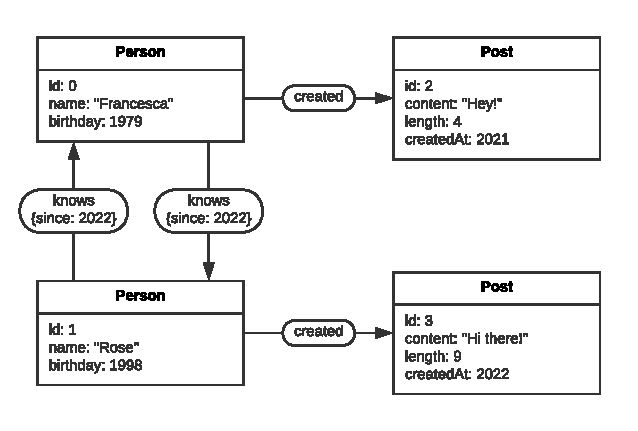
\includegraphics{figures/pg.pdf}
  \caption[A property graph representing a small movie database]{A property graph consisting of 5 nodes and 5 edges, representing a small movie database. Nodes and edges are given identifiers (in blue circles) in order to refer to them in text.}
  \label{fig:pg}
\end{figure}

An example of a property graph is given in \autoref{fig:pg}. Nodes are drawn as boxes, and edges are drawn as arrows. Node labels are written in the top compartment, and node properties are written in the bottom compartment. Edge labels are written inside a pill and edge properties are surrounded by `\{' and `\}', which may be omitted when an edge has no properties.

The example of \autoref{fig:pg} can be mapped to our formal property graph model in the following way:
\begin{align*}
  &N = \{n_1, n_2, n_3, n_4, n_5\}\\
  &E = \{e_1, e_2, e_3, e_4, e_5\}\\
  &\rho(e_1) = (n_1, n_3) \quad \rho(e_2) = (n_2, n_3) \quad \rho(e_3) = (n_4, n_3) \quad \rho(e_4) = (n_4, n_3) \quad \rho(e_5) = (n_3, n_5)\\
  &\lambda(n_1) = \{\texttt{Person}, \texttt{Actor}, \texttt{Director}\} \quad \lambda(n_2) = \{\texttt{Person}, \texttt{Director}\} \quad \lambda(n_3) = \{\texttt{Movie}\}\\
  &\lambda(n_4) = \{\texttt{User}\} \quad \lambda(n_5) = \{\texttt{Genre}\} \quad \lambda(e_1) = \{\texttt{ACTED}\} \quad \lambda(e_2) = \{\texttt{DIRECTED}\}\\
  &\lambda(e_3) = \{\texttt{RATED}\} \quad \lambda(e_4) = \{\texttt{RATED}\} \quad \lambda(e_5) = \{\texttt{IN\_GENRE}, \texttt{CLASSIC}\}\\
  &\pi(n_1) = \langle \texttt{born} : \texttt{1930-05-31},\;\texttt{name} : \texttt{Clint Eastwood},\;\texttt{url} : \texttt{person/190} \rangle\\
  &\pi(n_2) = \langle \texttt{born} : \texttt{1929-01-03},\;\texttt{name} : \texttt{Sergio Leone},\;\texttt{url} : \texttt{person/4385} \rangle\\
  &\pi(n_3) = \langle \texttt{rating} : \texttt{8.9},\;\texttt{title} : \texttt{The Good, the Bad and the Ugly},\;\texttt{url} : \texttt{movie/429},\\
  &\quad\texttt{year} : \texttt{1966} \rangle \quad \pi(n_4) = \langle \texttt{name} : \texttt{Deborah} \rangle \quad \pi(n_5) = \langle \texttt{name} : \texttt{Western} \rangle\\
  &\pi(e_1) = \langle \texttt{role} : \texttt{Blondie} \rangle \quad \pi(e_2) = \langle\rangle \quad \pi(e_3) = \langle \texttt{timestamp} : \texttt{1970-01-14},\;\texttt{rating} : \texttt{2.0}\rangle\\
  &\pi(e_4) = \langle \texttt{timestamp} : \texttt{1979-07-31},\;\texttt{rating} : \texttt{5.0}\rangle \quad \pi(e_5) = \langle\rangle
\end{align*}

\chapter{Property Graph Schemas}
\label{ch:pg-schema}

In this chapter, we design a schema model for property graphs, and provide a formal specification. We provide a set of first-order logic rules which determine whether a property graph conforms to a schema.

A schema should allow modeling of all kinds of entities and their relationships. A more expressive schema language enables the specification of more complex constraints, but this may come at the cost of greater research and engineering effort, as well as worse runtime performance. This needs to be balanced in the design of our schema model.

To explore the schema features that are commonly used in practice, let us look at some existing data modeling techniques. As a baseline, we consider the Entity--Relationship (ER) model as proposed by~\citet{chen1976entity}. This model incorporates entities, relationships, attributes, and values. An \emph{entity} is a ``thing'' that can be uniquely identified, a \emph{relationship} is an association between entities, and an \emph{attribute--value} pair represents information about an entity or relationship. Furthermore, an entity may have a \emph{role} in a relationship, such as ``white'' or ``black'' in a chess match relationship. These are the concepts underlying many conceptual data modeling methods in use today.

After the original specification, the ER model has been extended in various ways. For example, a notation which introduced cardinality constraints, optionality, and subtype relations was developed by~\citet{barker1990entity}. With these additions, we can create a more nuanced data model which fits the real world more closely.

In the next section, we first establish a basic definition of property graph schema, which we then extend with additional features such as cardinality constraints (\autoref{sec:cardinality}) and optional properties (\autoref{sec:optional-properties}).

\section{Basic Definition}

In this section, we define a notion of property graph schema which incorporates the basic features of the ER model: entities, relationships, attributes, and values. \autoref{tab:er-pg} shows how the basic elements of the ER model can be mapped to the property graph model. Note that there are no named roles in the property graph model, but the direction of an edge does allow the distinction between the source and target of an edge. Conversely, the edge direction can be represented using roles in the ER model.

\begin{table}[t]
  \centering
  \begin{tabular}{ll}
    \hline
    \textbf{ER}  & \textbf{PG}     \\
    \hline
    Entity       & Node            \\
    Relationship & Edge            \\
    Attribute    & Property name   \\
    Value        & Value           \\
    Role*        & Edge direction* \\
    \hline
  \end{tabular}
  \caption[Mapping between entity--relationship and property graph concepts]{Mapping between entity--relationship (ER) and property graph (PG) concepts. $*$: roles and edge direction can be used for similar purposes, but are not equivalent.}
  \label{tab:er-pg}
\end{table}

To formally define property graph schemas and schema conformance, we first assume the existence of a set of property types $\mathcal{T}$. Next, we introduce a number of supporting concepts.

\begin{definition}[Basic property conformance]
  \label{def:property-conformance-basic}
  For each property type $\ptype \in \ptypes$ there is a set $\sem{\ptype} \subseteq \mathcal{V}$ that contains all property values that \emph{conform} to the type $\ptype$.
\end{definition}

The concept of property type is similar to a \emph{value set} in the ER model. Value sets and property types are used to specify which values may be associated with an attribute, or which values a property is allowed to have\footnote{Note the subtle difference in terminology: an ER attribute has a value, whereas a property has a name and a value.}. A minor difference is that \citet{chen1976entity} postulates that values from different value sets can be equivalent, while we do not have a notion of value equivalence.

\begin{definition}[Basic record type]
  \label{def:record-type-basic}
  A \emph{record type} is a finite partial function $\rtype : \mathcal{N} \pto \ptypes$ that maps some property names to a property type. We denote such record types as $\langle a_1 : \ptype_1, \ldots, a_n : \ptype_n \rangle$.
\end{definition}

\begin{definition}[Basic record conformance]
  \label{def:record-conformance-basic}
  We say that a record $r$ \emph{conforms} to a record type $\rtype$, denoted $r \in \sem{\rtype}$, if for each property name $k \in \mathcal{N}$ it holds that (1) $r(k)$ is defined iff $\rtype(k)$ is defined and (2) $r(k) \in \sem{\rtype(k)}$ if $r(k)$ and $\rtype(k)$ are defined.
\end{definition}

\begin{definition}[Object type]
  \label{def:object-type}
  An \emph{object type} is a pair $\otype = (L, \rtype)$ where $L \subseteq \mathcal{L}$ is a finite set of labels and and $\rtype$ a record type.
  % We denote such object types also simply as $L\rtype$ or $\{ l_1 \ldots l_k \} \langle a_1 : \rtype_1, \ldots, a_n : \rtype_n \rangle$.
  The set of all object types is denoted as $\otypes$.
\end{definition}

\begin{definition}[Object conformance]
  \label{def:object-conformance}
  Let $G = (N, E, \rho, \lambda, \pi)$ be a property graph and $\otype = (L, \rtype)$ an object type. The set of objects that \emph{conform} to $\otype$ is defined as $\sem{\otype} = \{o \in N \cup E \mid \lambda(o) = L \wedge \pi(o) \in \sem{\rtype}\}$.
\end{definition}

\begin{definition}[Basic property graph schema]
  \label{def:pg-schema-basic}
  A \emph{property graph schema} is a tuple $$S = (N, E, \rho, \omega)$$ where
  \begin{itemize}
    \item $N$ is a finite set of schema nodes;
    \item $E$ is a finite set of schema edges such that $N \cap E = \emptyset$;
    \item $\rho : E \to (N \times N)$ is a total function mapping schema edges to ordered pairs of schema nodes;
    \item $\omega : (N \cup E) \to \otypes$ is a total function mapping schema objects to object types.
  \end{itemize}
\end{definition}

An example of a basic property graph schema is given in \autoref{fig:pg-schema-basic}. The similarity between property graphs and schemas allows us to visualize and think about them using the same mental model. Schema nodes and edges are drawn in the same way as data graphs, but properties are associated with types rather than concrete values.

\begin{figure}[t]
  \centering
  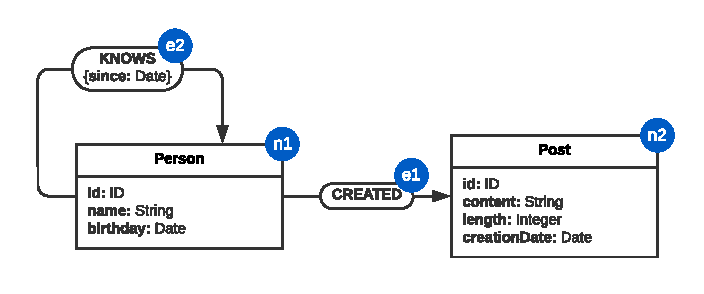
\includegraphics{figures/pg-schema-basic.pdf}
  \caption{A basic property graph schema.}
  \label{fig:pg-schema-basic}
\end{figure}

Note that a property graph schema can be simulated by a property graph if we allow properties to take property types as values, i.e. $\ptypes \subseteq \mathcal{V}$. Then we let $\lambda$ and $\pi$ take the role of $\omega$: for all schema objects $o$ in the property graph schema, if $\omega(o) = (L, \rtype)$ then $\lambda(o) = L$ and $\pi(o) = \rtype$.

The example of \autoref{fig:pg-schema-basic} can be mapped to our basic property graph schema model in the following way:
\begin{align*}
  &N = \{n_1, n_2\}\\
  &E = \{e_1, e_2\}\\
  &\rho(e1) = (n_1, n_2) \quad \rho(e_2) = (n_1, n_1)\\
  &\lambda(n_1) = \{\texttt{Person}\} \quad \lambda(n_2) = \{\texttt{Person}\} \quad \lambda(e_1) = \{\texttt{CREATED}\} \quad \lambda(e_2) = \{\texttt{KNOWS}\}\\
  &\omega(n_1) = (\{\texttt{Person}\}, \langle \texttt{id} : \texttt{ID},\;\texttt{name} : \texttt{String},\;\texttt{birthday} : \texttt{Date} \rangle)\\
  &\omega(n_2) = (\{\texttt{Post}\}, \langle \texttt{id} : \texttt{ID},\;\texttt{content} : \texttt{String},\;\texttt{length} : \texttt{Integer},\;\texttt{creationDate} : \texttt{Date} \rangle)\\
  &\omega(e_1) = (\{\texttt{CREATED}\}, \langle\rangle) \quad \omega(e_2) = (\{\texttt{KNOWS}\}, \langle \texttt{since} : \texttt{Date} \rangle)
\end{align*}
Here, we use \texttt{ID}, \texttt{String}, \texttt{Date}, and \texttt{Integer} to denote property types. Their semantics may depend on the specific implementation. For example, $\sem{\texttt{ID}}$ could be the set of all UUIDs\footnote{\url{https://www.rfc-editor.org/rfc/rfc4122}}, and $\sem{\texttt{Integer}}$ could be the set of all 32-bit integers.

We can relate our schema formalism to the ER model once again. Our definitions of schema nodes and schema edges are analogous to the concepts of \emph{entity set} and \emph{relationship set}, respectively. Entity sets and schema nodes represent classes of entities that have something in common, whereas relationship sets and schema edges represent classes of relationships. \autoref{tab:er-pg-schema} summarizes the relationship between the ER model and our schema formalism.

\begin{table}[t]
  \centering
  \begin{tabular}{ll}
    \hline
    \textbf{ER}      & \textbf{PG Schema} \\
    \hline
    Entity set       & Schema node        \\
    Relationship set & Schema edge        \\
    Value set        & Property type*     \\
    \hline
  \end{tabular}
  \caption[Mapping between entity--relationship and property graph schema concepts]{Mapping between entity--relationship (ER) and property graph (PG) schema concepts. $*$: strictly speaking, a property type $\ptype$ is not a set, but $\sem{\ptype}$ is.}
  \label{tab:er-pg-schema}
\end{table}

To make it easier to reason about objects conforming to schema objects, we introduce the \emph{conformance relation}.

\begin{definition}[Conformance relation]
  Given a property graph $$G = (N, E, \rho, \lambda, \pi)$$ and a property graph schema $$S = (N', E', \rho', \omega)$$ we define the binary \emph{conformance relation} $$\conf \; = \{(o, o') \in (N \cup E) \times (N' \cup E') \mid o \in \sem{\omega(o')}\}$$ We say that an object $o$ \emph{conforms} to a schema object $o'$ if and only if $o \conf o'$.
\end{definition}

Finally, we define what it means for a property graph to \emph{conform} to a schema.

\begin{definition}[Basic schema conformance]
  \label{def:schema-conformance-basic}
  Given a property graph $$G = (N, E, \rho, \lambda, \pi)$$ and a property graph schema $$S = (N', E', \rho', \omega)$$ we say that $G$ \emph{conforms} to $S$ if and only if all of the following rules hold.

  \begin{enumerate}
    \item\label{rule:basic-node}
    Every node $n$ conforms to some schema node $n'$:
    \begin{align*}
       & \forall n \in N \; \exists n' \in N' : n \conf n'
    \end{align*}

    \item\label{rule:basic-edge}
    Every edge $e$ conforms to some schema edge $e'$, and the source and target nodes of $e$ conform to the respective endpoints of $e'$:
    \begin{align*}
       & \forall e \in E \; \exists e' \in E' :                      \\
       & \quad e \conf e' \wedge \src(\rho(e)) \conf \src(\rho'(e'))
      \wedge \trg(\rho(e)) \conf \trg(\rho'(e'))
    \end{align*}
  \end{enumerate}
\end{definition}

Intuitively, \autoref{rule:basic-node} specifies the types of nodes that are allowed to exist in the graph. If there exists a node in the graph that is not specified in the schema, the graph does not conform. \autoref{rule:basic-edge} similarly specifies the allowed types of edges. In contrast to \autoref{rule:basic-node}, it looks not only at the properties of the edge itself, but also at the source and target nodes. This prevents a node from having an edge that is not explicitly allowed, even if that edge itself does conform to some schema edge.

\autoref{fig:conformance-basic} contains some examples of property graphs which are validated against the schema of \autoref{fig:pg-schema-basic}. In particular, \autoref{fig:conformance-basic-in} shows a case that we might want to prevent (a \texttt{Post} with no creator), but the current schema formalism cannot express this. In general, it is not possible to specify that an edge is mandatory under these definitions. In the next subsection, we introduce a notion of cardinality constraints which makes this possible.

\begin{figure}[t]
  \centering
  \begin{subfigure}[t]{0.45\textwidth}
    \centering
    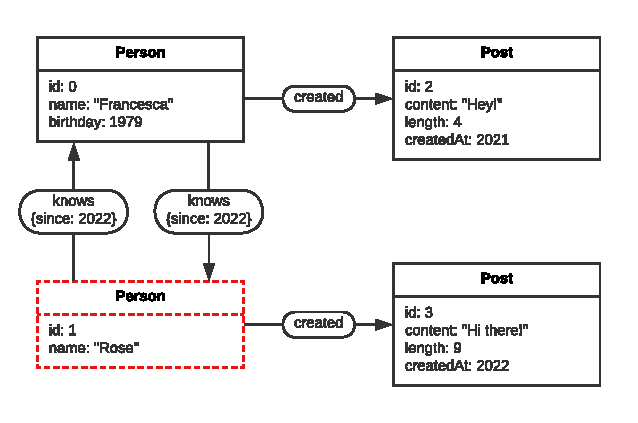
\includegraphics[width=\textwidth]{figures/conformance-basic-node.pdf}
    \caption{A \texttt{Person} is missing a \texttt{birthday}, which violates \autoref{rule:basic-node}.}
    \label{fig:conformance-basic-node}
  \end{subfigure}
  \hfill
  \begin{subfigure}[t]{0.45\textwidth}
    \centering
    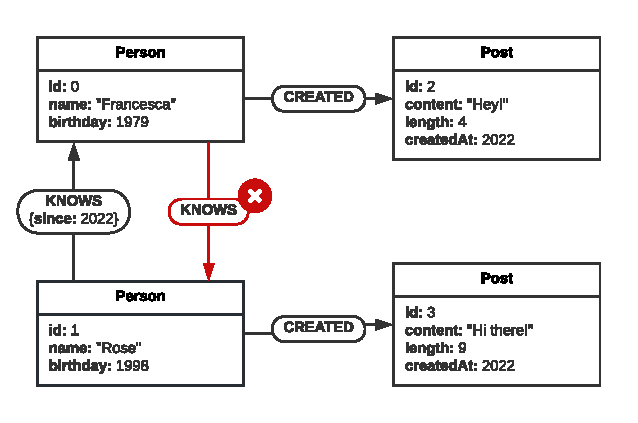
\includegraphics[width=\textwidth]{figures/conformance-basic-edge.pdf}
    \caption{A \texttt{KNOWS} edge is missing a \texttt{since} property, which violates \autoref{rule:basic-edge}.}
    \label{fig:conformance-basic-edge}
  \end{subfigure}

  \vskip\baselineskip

  \begin{subfigure}[t]{0.45\textwidth}
    \centering
    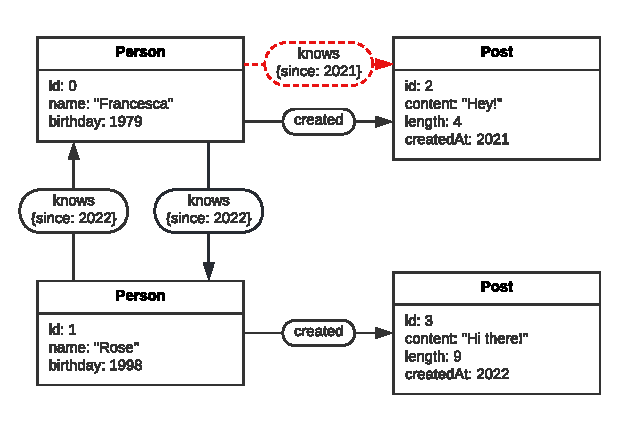
\includegraphics[width=\textwidth]{figures/conformance-basic-edge-target.pdf}
    \caption{The target of a \texttt{KNOWS} edge is not a \texttt{Person}, which violates \autoref{rule:basic-edge}.}
    \label{fig:conformance-basic-edge-target}
  \end{subfigure}
  \hfill
  \begin{subfigure}[t]{0.45\textwidth}
    \centering
    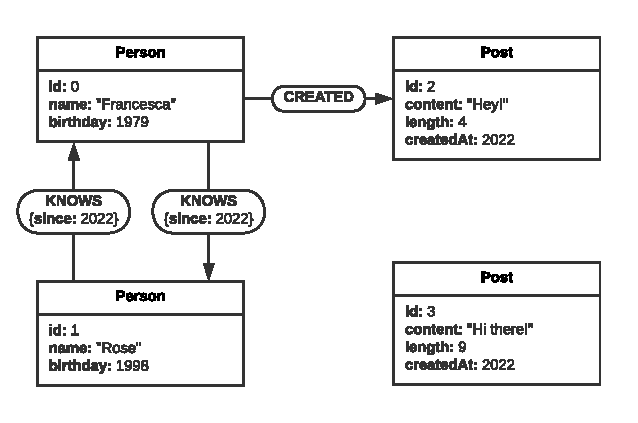
\includegraphics[width=\textwidth]{figures/conformance-basic-in.pdf}
    \caption{Conforms to the schema. A \texttt{Post} is missing an incoming \texttt{CREATED} edge, but this does not violate any rules.}
    \label{fig:conformance-basic-in}
  \end{subfigure}

  \caption[Property graphs validated against \autoref{fig:pg-schema-basic}]{Examples of property graphs validated against the schema of \autoref{fig:pg-schema-basic}. Violating nodes and edges are marked and have a red outline.}
  \label{fig:conformance-basic}
\end{figure}

\section{Cardinality Constraints}
\label{sec:cardinality}

We first introduce a generalization of the existential quantifier which enables counting the number of distinct variables that satisfy a predicate.

\begin{definition}[Counting quantifier]
  The \emph{counting quantifier} is defined as follows. Given two numbers $n, m \in \N$, a predicate $P$, and a set $X$, define
  \begin{itemize}
    \item $\exists^{\geq n} x \in X : P(x) \equiv \exists x_1, \ldots, x_n \in X : P(x_1) \wedge \ldots \wedge P(x_n) \wedge \forall 1 \leq i < j \leq n : x_i \neq x_j$;
    \item $\exists^{\leq n} x \in X : P(x) \equiv \exists x_1, \ldots, x_n, x_{n+1}, \ldots, x_k \in X : P(x_1) \wedge \ldots \wedge P(x_k) \implies \forall n < i < j \leq k : x_i = x_j$;
    \item $\exists^{[n, m]} x \in X : P(x) \equiv \exists^{\geq n} x \in X : P(x) \wedge \exists^{\leq m} x' \in X : P(x')$;
    \item $\exists^{[n, *]} x \in X : P(x) \equiv \exists^{\geq n} x \in X : P(x)$.
  \end{itemize}

  Here, the $\equiv$ operator denotes logical equivalence.
\end{definition}

Next, we introduce the notion of a \emph{cardinality constraint}.

\begin{definition}[Cardinality constraint]
  \label{def:cardinality-constraint}
  A \emph{cardinality constraint} is an ordered pair of intervals $([n_1, m_1], \, [n_2, m_2])$ where $n_1, n_2 \in \N$ and $m_1, m_2 \in \N^*$ with $\N = \{0, 1, 2, \ldots\}$ and $\N^* = \N \cup \{*\}$. The set of all cardinality constraints is denoted as $\mathcal{C}$.
\end{definition}

The two intervals of a cardinality constraint apply to the source and target of an edge, respectively. We also use the functions $\src$ and $\trg$ to refer to the first and second interval of a cardinality constraint, i.e. $\src([n_1, m_1], \, [n_2, m_2]) = [n_1, m_1]$ and $\trg([n_1, m_1], \, [n_2, m_2]) = [n_2, m_2]$.

Next, we revise the definitions of property graph schema and schema conformance, making use of our newly defined cardinality constraints. The following definitions subsume \autoref{def:pg-schema-basic} and~\ref{def:schema-conformance-basic}.

\begin{definition}[Property graph schema]
  \label{def:pg-schema}
  A \emph{property graph schema} is a tuple $$S = (N, E, \rho, \omega, \eta)$$ where
  \begin{itemize}
    \item $N$ is a finite set of schema nodes;
    \item $E$ is a finite set of schema edges such that $N \cap E = \emptyset$;
    \item $\rho : E \to (N \times N)$ is a total function mapping schema edges to ordered pairs of schema nodes;
    \item $\omega : (N \cup E) \to \otypes$ is a total function mapping schema objects to object types;
    \item $\eta : E \to \mathcal{C}$ is a total function mapping schema edges to cardinality constraints.
  \end{itemize}
\end{definition}

An example of a property graph schema with cardinality constraints is given in \autoref{fig:pg-schema}. Intervals such as $[n, m]$ are written as $n..m$, and $[n, n]$ is written simply as $n$, following notation established in UML~\citep{uml}. Furthermore, we use the ``look-across'' notation (as opposed to ``look-here''), meaning that the interval indicates the minimum and maximum number of edges that the node on the other side of the edge must participate in. Contrary to some data modeling diagram conventions, the arrow head is unrelated to cardinality, instead it specifies the direction of an edge. Note  that every property graph that conforms to \autoref{fig:pg-schema-basic} also conforms to \autoref{fig:pg-schema}, but not the other way around.

\begin{figure}[t]
  \centering
  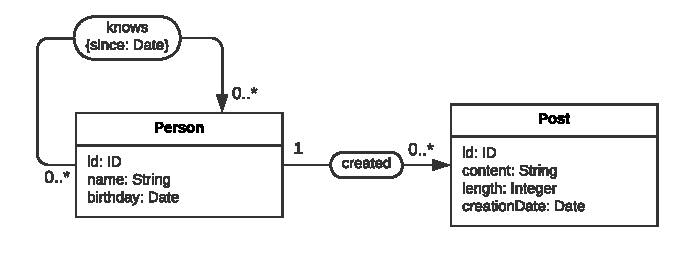
\includegraphics{figures/pg-schema.pdf}
  \caption[A property graph schema with cardinality constraints]{A property graph schema with cardinality constraints.}
  \label{fig:pg-schema}
\end{figure}

The example of \autoref{fig:pg-schema} can be mapped to our property graph schema model in the following way:
\begin{align*}
  &N = \{n_1, n_2\}\\
  &E = \{e_1, e_2\}\\
  &\rho(e1) = (n_1, n_2) \quad \rho(e_2) = (n_1, n_1)\\
  &\lambda(n_1) = \{\texttt{Person}\} \quad \lambda(n_2) = \{\texttt{Person}\} \quad \lambda(e_1) = \{\texttt{CREATED}\} \quad \lambda(e_2) = \{\texttt{KNOWS}\}\\
  &\omega(n_1) = (\{\texttt{Person}\}, \langle \texttt{id} : \texttt{ID},\;\texttt{name} : \texttt{String},\;\texttt{birthday} : \texttt{Date} \rangle)\\
  &\omega(n_2) = (\{\texttt{Post}\}, \langle \texttt{id} : \texttt{ID},\;\texttt{content} : \texttt{String},\;\texttt{length} : \texttt{Integer},\;\texttt{creationDate} : \texttt{Date} \rangle)\\
  &\omega(e_1) = (\{\texttt{CREATED}\}, \langle\rangle) \quad \omega(e_2) = (\{\texttt{KNOWS}\}, \langle \texttt{since} : \texttt{Date} \rangle)\\
  &\eta(e_1) = ([1, 1], [0, *]) \quad \eta(e_2) = ([0, *], [0, *])
\end{align*}
Next, we redefine schema conformance, taking cardinality constraints into account. This definition subsumes \autoref{def:schema-conformance-basic}.

\begin{definition}[Schema conformance]
  \label{def:schema-conformance}
  Given a property graph $$G = (N, E, \rho, \lambda, \pi)$$ and a property graph schema $$S = (N', E', \rho', \omega, \eta)$$ we say that $G$ \emph{conforms} to $S$ if and only if all of the following rules hold.

  \begin{enumerate}
    \item\label{rule:node}
    Every node $n$ conforms to some schema node $n'$:
    \begin{align*}
       & \forall n \in N \; \exists n' \in N' : n \conf n'
    \end{align*}

    \item\label{rule:edge}
    Every edge $e$ conforms to some schema edge $e'$, and the source and target nodes of $e$ conform to the respective endpoints of $e'$:
    \begin{align*}
       & \forall e \in E \; \exists e' \in E' :                      \\
       & \quad e \conf e' \wedge \src(\rho(e)) \conf \src(\rho'(e'))
      \wedge \trg(\rho(e)) \conf \trg(\rho'(e'))
    \end{align*}

    \item\label{rule:out}
    If a node $n$ conforms to the source of a schema edge $e'$, it must have the right number of outgoing edges of the right type:
    \begin{align*}
       & \forall n \in N \; \forall e' \in E' :                                                        \\
       & \quad \big[n \conf \src(\rho(e')) \implies \exists^{\trg(\eta(e'))} e \in E :                 \\
       & \quad\quad e \conf e' \wedge \src(\rho(e)) = n \wedge \trg(\rho(e)) \conf \trg(\rho(e'))\big]
    \end{align*}

    \item\label{rule:in}
    If a node $n$ conforms to the target of a schema edge $e'$, it must have the right number of incoming edges of the right type:
    \begin{align*}
       & \forall n \in N \; \forall e' \in E' :                                                        \\
       & \quad \big[n \conf \trg(\rho(e')) \implies \exists^{\src(\eta(e'))} e \in E :                 \\
       & \quad\quad e \conf e' \wedge \src(\rho(e)) \conf \src(\rho(e')) \wedge \trg(\rho(e)) = n\big]
    \end{align*}
  \end{enumerate}
\end{definition}

Compared to \autoref{def:schema-conformance-basic}, \autoref{rule:node} and \ref{rule:edge} are unchanged, while \autoref{rule:out} and \ref{rule:in} enforce cardinality constraints on edges. With these new rules, we can enforce mandatory edges, i.e. a cardinality constraint of ``at least one''.

\autoref{fig:conformance} contains some examples of property graphs which are validated against the schema of \autoref{fig:pg-schema}, taking into account the new rules.

\begin{figure}[t]
  \centering
  \begin{subfigure}[t]{0.45\textwidth}
    \centering
    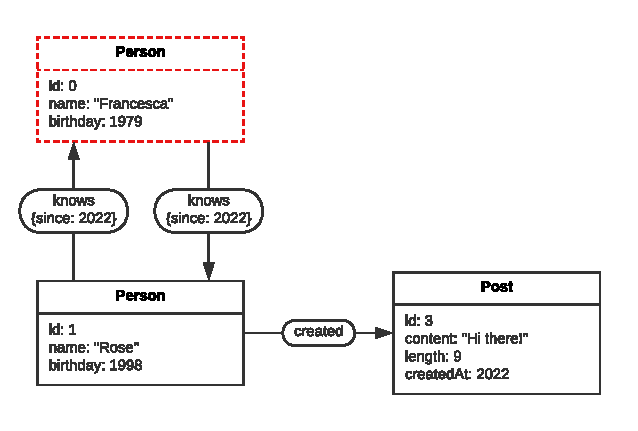
\includegraphics[width=\textwidth]{figures/conformance-out.pdf}
    \caption{Conforms to the schema. A \texttt{Person} is allowed to have created 0 \texttt{Post}s.}
    \label{fig:conformance-node}
  \end{subfigure}
  \hfill
  \begin{subfigure}[t]{0.45\textwidth}
    \centering
    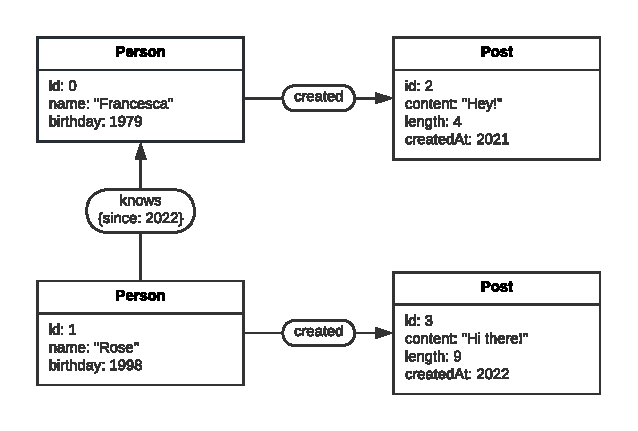
\includegraphics[width=\textwidth]{figures/conformance-out-2.pdf}
    \caption{Conforms to the schema. A \texttt{Person} is allowed to have no outgoing \texttt{KNOWS} edges.}
    \label{fig:conformance-edge}
  \end{subfigure}

  \vskip\baselineskip

  \begin{subfigure}[t]{0.45\textwidth}
    \centering
    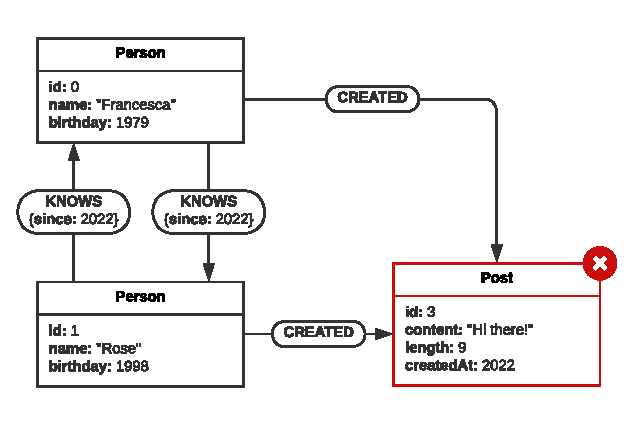
\includegraphics[width=\textwidth]{figures/conformance-too-many-in.pdf}
    \caption{This \texttt{Post} has too many incoming \texttt{CREATED} edges, which violates \autoref{rule:in}.}
    \label{fig:conformance-edge-target}
  \end{subfigure}
  \hfill
  \begin{subfigure}[t]{0.45\textwidth}
    \centering
    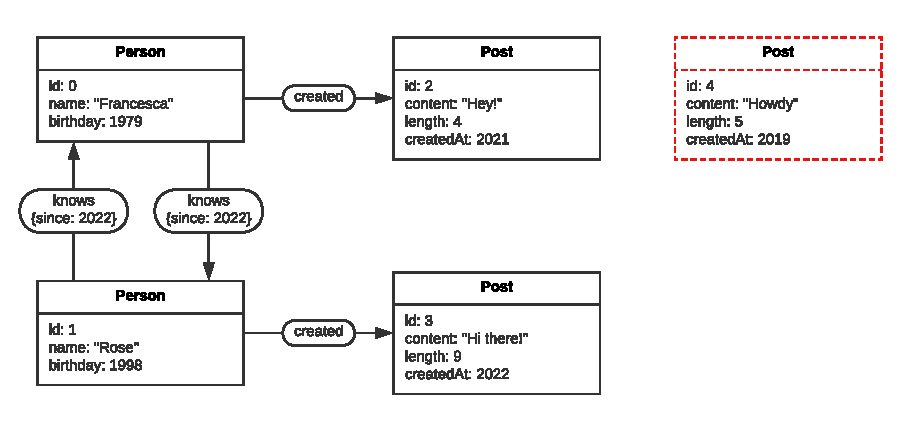
\includegraphics[width=\textwidth]{figures/conformance-in.pdf}
    \caption{A \texttt{Post} is missing an incoming \texttt{CREATED} edge, which violates \autoref{rule:in}.}
    \label{fig:conformance-out}
  \end{subfigure}

  \caption[Property graphs validated against \autoref{fig:pg-schema}]{Examples of property graphs validated against the schema of \autoref{fig:pg-schema}. Violating nodes and edges have are marked and have a red outline.}
  \label{fig:conformance}
\end{figure}

\section{Optional Properties}
\label{sec:optional-properties}

We revise the definition of record by adding a special property value $\undefined$, which indicates that the value of a property is not defined. The following definitions subsume \autoref{def:record-basic}, \ref{def:property-conformance-basic}, \ref{def:record-type-basic}, and \ref{def:record-conformance-basic}.

\begin{definition}[Record]
  \label{def:record}
  A \emph{record} is a total function $r : \mathcal{N} \to \mathcal{V} \cup \{\undefined\}$ that maps property names to property values or the special value $\undefined$. We denote such records as $\langle n_1 : v_1, \ldots, n_k : v_k \rangle$. The set of all records is denoted as $\mathcal{R}$.
\end{definition}

For a record $r$ and a property name $k \in \mathcal{N}$ such that $r(k)$ was previously undefined, we now say $r(k) = \undefined$. This can be seen as the ``default'' value of a property.

We adjust the definitions of property conformance, record type, and record conformance accordingly.

\begin{definition}[Property conformance]
  \label{def:property-conformance}
  For each property type $\ptype \in \ptypes$ there is a set $\sem{\ptype} \subseteq \mathcal{V} \cup \{\undefined\}$ that contains all property values that \emph{conform} to the type $\ptype$. We say $\ptype$ is \emph{optional} iff $\undefined \in \sem{\ptype}$. We use the notation $\ptype?$ to mark a property as optional, i.e. $\sem{\ptype?} = \sem{\ptype} \cup \{ \undefined \}$.
\end{definition}

\begin{definition}[Record type]
  \label{def:record-type}
  A \emph{record type} is a total function $\rtype : \mathcal{N} \to \ptypes$ that maps property names to property types. We denote such record types as $\langle n_1 : \ptype_1, \ldots, n_k : \ptype_k \rangle$.
\end{definition}

\begin{definition}[Record conformance]
  \label{def:record-conformance}
  We say that a record $r$ \emph{conforms} to a record type $\rtype$, denoted $r \in \sem{\rtype}$, if and only if for each property name $k \in \mathcal{N}$ it holds that $r(k) \in \sem{\rtype(k)}$.
\end{definition}

An example of a schema containing an optional property is shown in \autoref{fig:optional-property}. This examples illustrates that optional properties may be omitted, but if they are present, they must have a value of the right type.

\begin{figure}[t]
  \centering
  \begin{subfigure}[t]{0.8\textwidth}
    \centering
    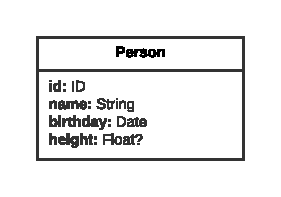
\includegraphics[scale=0.75]{figures/pg-schema-optional-prop.pdf}
    \caption{A schema consisting of a single schema node.}
  \end{subfigure}
  \hfill
  \begin{subfigure}[t]{0.8\textwidth}
    \centering
    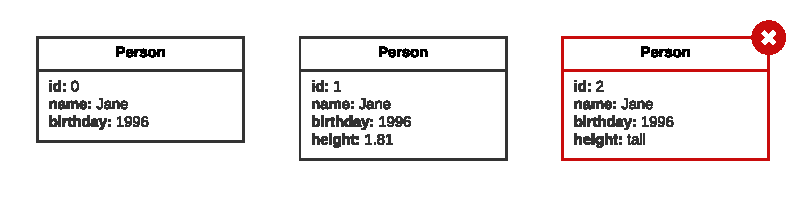
\includegraphics[scale=0.75]{figures/conformance-optional-prop.pdf}
    \caption{A property graph consisting of three disconnected nodes. Properties with a value of $\undefined$ are not shown. The node with \texttt{id}~:~\texttt{2} violates \autoref{rule:node} because the \texttt{height} property value is of the wrong type.}
  \end{subfigure}
  \caption[A property graph validated against a schema with an optional property]{A property graph validated against a schema with an optional property.}
  \label{fig:optional-property}
\end{figure}

\section{Open Record Types}

It may be desirable to allow a record to have properties with any name or any value. Such \emph{open record types} can already be expressed under the current definitions. For a record type $\rtype$, we can allow properties with any name by setting $\rtype(k) = \ptype?$ for all (previously unspecified) property names $k \in \mathcal{N}$, where $\ptype$ is an arbitrary property type. Note that there may be infinitely many such $k$, so in practice we may want to have a special syntax to express this. We can allow these properties to have any value by choosing a $\ptype$ such that $\sem{\ptype} = \mathcal{V}$, or we can restrict them to a subset of $\mathcal{V}$.

An example of a schema containing an open record type is shown in \autoref{fig:open-record}. An open record type allows properties with any name, but still requires explicitly defined properties to be of the right type.

\begin{figure}[t]
  \centering
  \begin{subfigure}[t]{0.8\textwidth}
    \centering
    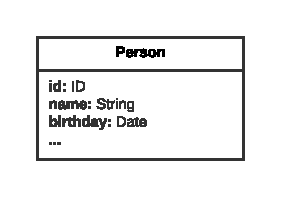
\includegraphics[scale=0.75]{figures/pg-schema-open-record.pdf}
    \caption{A schema consisting of a single schema node. Open records are indicated with \ldots at the bottom of the container.}
  \end{subfigure}
  \hfill
  \begin{subfigure}[t]{0.8\textwidth}
    \centering
    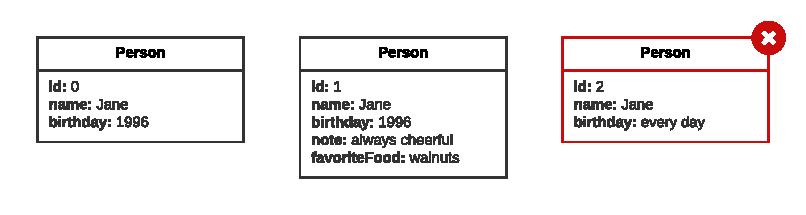
\includegraphics[scale=0.75]{figures/conformance-open-record.pdf}
    \caption{A property graph consisting of three disconnected nodes. The node with \texttt{id}~:~\texttt{2} violates \autoref{rule:node} because the \texttt{birthday} property value is of the the wrong type.}
  \end{subfigure}
  \caption[A property graph validated against a schema with an open record type]{A property graph validated against a schema with an open record type.}
  \label{fig:open-record}
\end{figure}

\section{Mapping Functionality to Rules}

In \autoref{ch:related-work}, we compared the capabilities of existing property graph schema implementation. We can now see how most of the features in \autoref{tab:pg-schema-databases} can be mapped to one of our conformance rules.

Mandatory and allowed properties are captured by our notion of record conformance (\autoref{def:record-conformance}), which corresponds to \autoref{rule:node}. Endpoint constraints correspond to \autoref{rule:edge}. Data type constraints are captured by our notion of object conformance (\autoref{def:object-conformance}), and correspond to \autoref{rule:node}. Cardinality constraints correspond to \autoref{rule:out} and \ref{rule:in}. Property uniqueness, label coexistence, and subtype relations are not covered by our formalism.

\chapter{Schema Validation in Practice}
\label{ch:practice}

Our property graph schema formalism is capable of expressing constraints in common conceptual data modeling methods. However, we have found that existing property graph database systems are limited in the kinds of constraints they can enforce, in particular cardinality constraints.

In this chapter, we describe how existing database systems can be extended to support all kinds of constraints that can be expressed with our schema formalism. Where possible, we make use of the schema functionality exposed by the database engine. For constraints that cannot be validated in this way, we provide graph queries.

We focus here on the same three databases we covered in \autoref{ch:related-work}: \emph{Neo4j}, \emph{JanusGraph}, and \emph{TigerGraph}. This is choice is motivated by the diversity of schema approaches employed by these systems. Neo4j's schemas are mostly inferred from data, whereas TigerGraph requires an explicit schema, and JanusGraph is schema-optional.

\section{Assumptions}

To reduce the complexity of the implementation, we assume that the set of labels of a schema object functionally determines the record type of that schema object. Recall from \autoref{ch:pg-schema} that every object must conform to a schema object (\autoref{rule:node} and \ref{rule:edge}). This implies that if an object has the same set of labels as a schema object, it must conform to that schema object (since there exists no schema object with the same label set and a different record type). We find that this assumption holds in many domains, including the datasets we study in \autoref{ch:experiment}.

Under this assumption, we can simplify the conformance rules. Informally:

% TODO: formalize this?
\begin{enumerate}
  \item
        \begin{enumerate}
          \item\label{rule:simp-node-labels}
          Every node has the same set of labels as some schema node.
          \item\label{rule:simp-node-mandatory-props}
          All mandatory properties exist on the node.
          \item\label{rule:simp-node-allowed-props}
          The node has no properties that are not allowed.
          \item\label{rule:simp-node-datatype}
          All node properties have a value of the right type.
        \end{enumerate}
  \item
        \begin{enumerate}
          \item\label{rule:simp-edge-labels}
          Every edge has the same set of labels as some schema edge.
          \item\label{rule:simp-edge-mandatory-props}
          All mandatory properties exist on the edge.
          \item\label{rule:simp-edge-allowed-props}
          The edge has no properties that are not allowed.
          \item\label{rule:simp-edge-datatype}
          All edge properties have a value of the right type.
          \item\label{rule:simp-edge-endpoints}
          Both endpoints of the edge have the right labels.
        \end{enumerate}
        \item\label{rule:simp-card-out}
        Every node has the right number of outgoing edges with the right labels.
        \item\label{rule:simp-card-in}
        Every node has the right number of incoming edges with the right labels.
\end{enumerate}

\section{Validation Variants}
\label{sec:variants}

We consider two variants of the schema validation problem:

\begin{itemize}
  \item \textbf{Binary validation:} given a graph and a schema, determine whether the graph conforms to the schema or not.
  \item \textbf{Full validation:} given a graph and a schema, find all graph objects which cause a violation of at least one of the rules of schema conformance.
\end{itemize}

While a binary validation method may be sufficient for some use cases, full validation is required when we want to explain why a graph does not conform. Binary validation is a strictly easier problem because we can stop as soon as we find a single violation, while full validation always needs to find all violations in the graph.

\section{Implementation}
\label{sec:implementation}

We describe how each conformance rule can be validated using the three databases in our scope. Both the binary and full validation variants are discussed. The full source code is available on GitHub\footnote{\url{https://github.com/nimobeeren/thesis}}.

\paragraph{Neo4j.} We start by using the built-in schema functionality that Neo4j offers. To ensure the existence of mandatory properties (\autoref{rule:simp-node-mandatory-props} and \ref{rule:simp-edge-mandatory-props}), we use Neo4j's \texttt{CONSTRAINT} functionality, which lets us specify which properties are mandatory for nodes and edges with a particular label set (Enterprise edition only). An example is given in \autoref{lst:neo4j-mandatory-props}.

\begin{figure}[H]
  \begin{lstlisting}[
    language=Cypher,
    caption={[Creation of Cypher constraints which require the existence of some mandatory properties on nodes]Creation of Cypher constraints which require the existence of some mandatory properties on \texttt{Movie} nodes.},
    label=lst:neo4j-mandatory-props
  ]
CREATE CONSTRAINT FOR (m:Movie) REQUIRE m.imdbId IS NOT NULL;
CREATE CONSTRAINT FOR (m:Movie) REQUIRE m.movieId IS NOT NULL;
CREATE CONSTRAINT FOR (m:Movie) REQUIRE m.title IS NOT NULL;
  \end{lstlisting}
\end{figure}

Next, we tackle the validation of the node and edge labels (\autoref{rule:simp-node-labels} and \ref{rule:simp-edge-labels}) using Cypher queries. Neo4j provides functions \texttt{db.labels()} and \texttt{db.relationshipTypes()}, which respectively return a list of all node and edge labels that exist in the database. Unfortunately, these functions do not tell us which \emph{combinations} of labels exist. Since nodes can have multiple labels, we must fall back to a \texttt{MATCH} query which checks that every node has one of the allowed combinations of labels (see \autoref{lst:neo4j-node-labels}). Since edges in Neo4j can only have one label (called a \emph{relationship type}), we can use \texttt{db.relationshipTypes()} to determine if there exist any edges with a label that is not allowed (see \autoref{lst:neo4j-edge-labels}). This is sufficient for binary validation, but if we want to find out precisely which edges have an illegal label, we again need to use a \texttt{MATCH} query.

\begin{figure}[H]
  \begin{lstlisting}[
    language=Cypher,
    caption={[A Cypher query to find all nodes that have a label set that is not allowed]A Cypher query to find all nodes that have a label set that is not allowed.},
    label=lst:neo4j-node-labels
  ]
WITH [["Actor", "Person"], ["Movie"], ["User"], ...] AS allowedNodeLabelSets
MATCH (n)
WHERE NOT labels(n) IN allowedNodeLabelSets
RETURN n
  \end{lstlisting}
\end{figure}
\vspace*{-8pt}
\begin{figure}[H]
  \begin{lstlisting}[
    language=Cypher,
    caption={[A Cypher query to check if there are any edge labels that are not allowed]A Cypher query to check if there are any edge labels that are not allowed. Note that this query returns a Boolean, and does not explain which edges have an illegal label.},
    label=lst:neo4j-edge-labels
  ]
WITH ["ACTED_IN", "DIRECTED", ...] AS allowedEdgeLabels
CALL db.relationshipTypes() YIELD relationshipType AS allTypes
RETURN all(type IN collect(allTypes) WHERE type IN allowedEdgeLabels)
  \end{lstlisting}
\end{figure}

Next, we look at the properties. The functions \texttt{db.schema.nodeTypeProperties()} and \texttt{db.schema.relTypeProperties()} provide useful information about the properties that exist on nodes and edges, as well as their data types. This allows us to determine if there are any nodes or edges that have properties that are not allowed (\autoref{rule:simp-node-allowed-props} and \ref{rule:simp-edge-allowed-props}), or have the wrong data type (\autoref{rule:simp-node-datatype} and \ref{rule:simp-edge-datatype}). See \autoref{lst:neo4j-allowed-props-binary} for an example of such a query. Again, if we want to find the violating objects, we need to use a \texttt{MATCH} query that scans all properties of all objects in the database. In that case, we use the \texttt{apoc.meta.type()} function (provided by the APOC library\footnote{\url{https://neo4j.com/labs/apoc/}}) to get the data type of a property at query-time. \autoref{lst:neo4j-allowed-props-full} shows an example.

\begin{figure}[H]
  \begin{lstlisting}[
    language=Cypher,
    caption={[A Cypher query to check if there are any nodes with properties that are not allowed or have the wrong data type]A Cypher query to check if there are any \texttt{User} nodes with properties that are not allowed or have the wrong data type. If the result is \texttt{true}, there are no violations.},
    label=lst:neo4j-allowed-props-binary
  ]
CALL db.schema.nodeTypeProperties() YIELD nodeLabels, propertyName, propertyTypes
WHERE "User" IN nodeLabels AND (
    NOT propertyName IN ["userId", "name"]
    OR propertyName = "userId" AND propertyTypes <> ["String"]
    OR propertyName = "name" AND propertyTypes <> ["String"]
)
RETURN count(nodeLabels) = 0
  \end{lstlisting}
\end{figure}
\vspace*{-8pt}
\begin{figure}[H]
  \begin{lstlisting}[
    language=Cypher,
    caption={[A Cypher query to find all nodes with properties that are not allowed or have the wrong data type]A Cypher query to find all \texttt{User} nodes with properties that are not allowed or have the wrong data type.},
    label=lst:neo4j-allowed-props-full
  ]
WITH {
    userId: "STRING",
    name: "STRING"
} AS propertyTypes
MATCH (n:User)
WHERE NOT all(pKey IN keys(n) WHERE pKey IN keys(propertTypes) AND apoc.meta.type(n[pKey]) = propertyTypes[pKey])
RETURN n
  \end{lstlisting}
\end{figure}

To check \autoref{rule:simp-edge-endpoints}, we do a \texttt{MATCH} query for every edge label, and look at the source and target nodes. For every edge, there must exist a schema edge such that the labels of the source and target in the data match the labels of the source and target in the schema.
% An example of such a query is shown in \autoref{lst:neo4j-endpoints}.

\begin{figure}[H]
  \begin{lstlisting}[
    language=Cypher,
    caption={[A Cypher query that finds all edges where the endpoints have the wrong label]A Cypher query that finds all \texttt{ACTED\_IN} edges where the endpoints have the wrong label. Note that the source node \texttt{n} may have additional labels.},
    label=lst:neo4j-endpoints
  ]
MATCH (n)-[e:ACTED_IN]->(m)
WHERE NOT "Actor" IN labels(n) OR NOT labels(m) = ["Movie"]
RETURN e;
  \end{lstlisting}
\end{figure}

Finally, we check the cardinality constraints (\autoref{rule:simp-card-out} and \ref{rule:simp-card-in}). Since the schemas of our datasets only contain ``one or more'' constraints, a simple \texttt{MATCH} query for each relevant node label is sufficient. See \autoref{lst:neo4j-mandatory-edges} for an example.
% If the cardinality constraint is more specific (say, exactly 3), then we can use the \texttt{size()} function to count the number of matches of the pattern.

\begin{figure}[H]
  \begin{lstlisting}[
    language=Cypher,
    caption={[A Cypher query to find nodes that are missing a mandatory edge]A Cypher query to find \texttt{ACTOR} nodes that are missing a mandatory \texttt{ACTED\_IN} edge.},
    label=lst:neo4j-mandatory-edges
  ]
MATCH (a:Actor)
WHERE NOT (a)-[:ACTED_IN]->(:Movie)
RETURN a;
  \end{lstlisting}
\end{figure}

To give the database engine the best opportunity to perform query optimization, the queries described here are merged as much as possible. These merged queries are then executed sequentially. This is particularly relevant for the binary variant, since it can terminate as soon as a single violation is found. For \texttt{MATCH} queries, we always return a value using \texttt{count(variable) = 0}. This theoretically allows the query to terminate early, but it is up to the query engine to implement this optimization.

\paragraph{JanusGraph.} The extensive set of schema features that JanusGraph provides allow us to specify most conformance rules at the time of schema definition, preventing any non-conforming data from being inserted. The complete set of allowed node and edge labels (\autoref{rule:simp-node-labels} and \ref{rule:simp-edge-labels}) are defined using \texttt{makeVertexLabel()} and \texttt{makeEdgeLabel()}. Because JanusGraph only allows a single label on an object, we concatenate the labels if more than one is present in the data. This does not affect the semantics (as long as the order of concatenation is consistent), since we only ever check for equality of label sets (see \autoref{def:object-conformance}).

For each edge label, the method \texttt{addConnection()} lets us specify the allowed labels of the edge endpoints (\autoref{rule:simp-edge-endpoints}). The maximum cardinality for an edge label is set with \texttt{multiplicity()}, but this does not provide any guarantees on minimum cardinality.

The complete set of allowed property names is defined using \texttt{makePropertyKey()}. Next, each label is mapped to a set of property names using \texttt{addProperties()}. This prevents objects from having properties that are not allowed (\autoref{rule:simp-node-allowed-props} and \ref{rule:simp-edge-allowed-props}). The data type of each property is defined using \texttt{dataType()} (\autoref{rule:simp-node-datatype} and \ref{rule:simp-edge-datatype}). In JanusGraph, there cannot exist two properties with the same name and different data type. If this is desired, the property name must be disambiguated, which could be achieved by prefixing it with the object label.

For an example of all of JanusGraph's built-in schema functions working together, have a look at \autoref{lst:janusgraph-schema}.

\begin{figure}[H]
  \begin{lstlisting}[
    language=Java,
    caption={[A fragment of the Recommendations schema, expressed using JanusGraph's schema methods]A fragment of the Recommendations schema, expressed using JanusGraph's schema methods. Mandatory properties and cardinality constraints cannot be validated in this way. The \texttt{Multiplicity.SIMPLE} configuration ensures there is no more than one \texttt{ACTED\_IN} edge between any given actor and movie.},
    label=lst:janusgraph-schema
  ]
// Vertex labels
VertexLabel Actor = mgmt.makeVertexLabel("Actor").make();
VertexLabel Movie = mgmt.makeVertexLabel("Movie").make();
// Edge labels
EdgeLabel ACTED_IN = mgmt.makeEdgeLabel("ACTED_IN").multiplicity(Multiplicity.SIMPLE).make();
// Edge connections
mgmt.addConnection(ACTED_IN, Actor, Movie);
// Property keys
PropertyKey nameKey = mgmt.makePropertyKey("name").dataType(String.class).make();
PropertyKey titleKey = mgmt.makePropertyKey("title").dataType(String.class).make();
PropertyKey revenueKey = mgmt.makePropertyKey("revenue").dataType(Long.class).make();
PropertyKey roleKey = mgmt.makePropertyKey("role").dataType(String.class).make();
// Property mapping
mgmt.addProperties(Actor, nameKey);
mgmt.addProperties(Movie, titleKey, revenueKey);
mgmt.addProperties(ACTED_IN, roleKey);
  \end{lstlisting}
\end{figure}

The remaining rules cannot be fully enforced by JanusGraph's schema, so we write queries to achieve this. Missing mandatory properties (\autoref{rule:simp-node-mandatory-props} and \ref{rule:simp-edge-mandatory-props}) are found using a combination of \texttt{hasLabel} and \texttt{hasNot} steps of the Gremlin query language (see \autoref{lst:janusgraph-mandatory-props}). For cardinality constraints, we leverage the fact that our schemas only have constraints of the form ``one or more''. We can validate these constraints using a combination of \texttt{hasLabel}, \texttt{outE}, and \texttt{inE} steps (see \autoref{lst:janusgraph-mandatory-edges}).

\begin{figure}[H]
  \begin{lstlisting}[
    language=Java,
    caption={[A Gremlin query to find nodes which are missing a mandatory property]A Gremlin query to find \texttt{User} nodes which are missing a mandatory \texttt{name} or \texttt{userId} property.},
    label=lst:janusgraph-mandatory-props
  ]
g.V().hasLabel("User").or(hasNot("name"), hasNot("userId"))
  \end{lstlisting}
\end{figure}
\vspace*{-8pt}
\begin{figure}[H]
  \begin{lstlisting}[
    language=Java,
    caption={[A Gremlin query to find nodes which are missing an outgoing edge]A Gremlin query to find \texttt{Actor} nodes which are missing an outgoing \texttt{ACTED\_IN} edge. Note that \texttt{ActorDirector} is the concatenation of the \texttt{Actor} and \texttt{Director} labels.},
    label=lst:janusgraph-mandatory-edges
  ]
g.V().hasLabel(P.within("Actor", "ActorDirector"))
    .not(outE("ACTED_IN"))
  \end{lstlisting}
\end{figure}

If we are only interested in the binary validation problem, we only need to determine whether the query result is empty. This is achieved using Java's \texttt{hasNext()} iterator method, which tells the query engine to stop traversing the graph as soon as one result has been found. To give the query engine the best chance of terminating early, we write the entire validation as a single disjunctive query. JanusGraph unfortunately does not allow a single query to range over all nodes and all edges, so instead we execute one query for nodes and one for edges, in sequence.

\paragraph{TigerGraph.} Before any data is loaded, TigerGraph requires specification of a schema describing all nodes, edges and their properties. This is done with a series of \texttt{CREATE VERTEX} and \texttt{CREATE EDGE} statements. Using these built-in schema capabilities, we can already guarantee conformance to some of our rules. Every node and edge has a label that appears in the schema (\autoref{rule:simp-node-labels} and \ref{rule:simp-edge-labels}) and has a fixed set of properties associated with that label (\autoref{rule:simp-node-allowed-props} and \ref{rule:simp-edge-allowed-props}). Every property has a fixed data type (\autoref{rule:simp-node-datatype} and \ref{rule:simp-edge-datatype}). Furthermore, every node type has a primary key. Finally, every edge type must specify a source and target node types (\autoref{rule:simp-edge-endpoints}).

\begin{figure}[H]
  \begin{lstlisting}[
    language=GSQL,
    caption={[A fragment of the Recommendations schema, expressed in TigerGraph's schema definition language]A fragment of the Recommendations schema, expressed in TigerGraph's schema definition language.},
    label=lst:tigergraph-schema
  ]
CREATE VERTEX Actor (
    PRIMARY_ID id STRING,
    name STRING
)
CREATE VERTEX Movie (
    PRIMARY_ID id STRING,
    title STRING,
    revenue INT
)
CREATE DIRECTED EDGE ACTED_IN (
    FROM Actor,
    TO Movie,
    role STRING
)
  \end{lstlisting}
\end{figure}

In TigerGraph, all properties must have a value as soon as the object is instantiated (there are no null values). When a value is missing, it is set to a default value, such as the empty string, the number 0, or the first of January 1970. While it is possible to prevent objects with missing values from being loaded, in some cases we may want to check for missing values in an existing database. To this end, we use a query to find all objects which have a mandatory property with the default value (validating \autoref{rule:simp-node-mandatory-props} and \ref{rule:simp-edge-mandatory-props}). If the default value naturally appears in valid data, then we use another indicator value. The query consists of a set of simple \texttt{SELECT-FROM-WHERE} patterns which range over all nodes and edges, as in \autoref{lst:tigergraph-mandatory-props}.

\begin{figure}[H]
  \begin{lstlisting}[
    language=GSQL,
    caption={[A GSQL query to find nodes which have a mandatory property with a default value]A GSQL query to find \texttt{Movie} and \texttt{User} nodes which have a mandatory property with a default value. All violating nodes are collected in the accumulator variable \texttt{@@violatingNodes}, which is returned at the end.},
    label=lst:tigergraph-mandatory-props
  ]
SetAccum<VERTEX> @@violatingNodes;

violatingMovies =
    SELECT movie
    FROM Movie:movie
    WHERE movie.imdbId == "" OR movie.movieId == ""
        OR movie.title == "";
    ACCUM @@violatingNodes += movie;

violatingUsers =
    SELECT user
    FROM User:user
    WHERE user.name == "" OR user.userId == "";
    ACCUM @@violatingNodes += user;

PRINT @@violatingNodes;
  \end{lstlisting}
\end{figure}

To cover the final remaining rules, cardinality constraints are validated using another query. For outgoing edges (\autoref{rule:simp-card-out}), we use the built-in \texttt{outdegree()} function, which returns the number of outgoing edges with a particular label for a given node (see \autoref{lst:tigergraph-mandatory-edges-out}). By default, TigerGraph maintains an index that stores these statistics for every node. For incoming edges (\autoref{rule:simp-card-in}), we use another TigerGraph feature known as an accumulator. This lets us compute the number of incoming edges for all relevant nodes in a single pass over the graph. Afterwards, the violating nodes are picked out (see \autoref{lst:tigergraph-mandatory-edges-in}).

\begin{figure}[H]
  \begin{lstlisting}[
    language=GSQL,
    caption={[A GSQL query to find nodes which are missing a outgoing edge]A GSQL query to find \texttt{Actor} nodes which are missing a outgoing \texttt{ACTED\_IN} edge.},
    label=lst:tigergraph-mandatory-edges-out
  ]
SELECT actor
FROM Actor:actor
WHERE actor.outdegree("ACTED_IN") == 0
  \end{lstlisting}
\end{figure}
\vspace*{-8pt}
\begin{figure}[H]
  \begin{lstlisting}[
    language=GSQL,
    caption={[A GSQL query to find nodes which are missing an incoming edge]A GSQL query to find \texttt{Post} nodes which are missing a incoming \texttt{CONTAINER\_OF} edge.},
    label=lst:tigergraph-mandatory-edges-in
  ]
SumAccum<int> @numContainerOf;
tmp =
    SELECT post
    FROM :n -(CONTAINER_OF>)- Post:post
    ACCUM post.@numContainerOf += 1;
violatingActors =
    SELECT post
    FROM Post:post
    WHERE post.@numContainerOf == 0
  \end{lstlisting}
\end{figure}

All TigerGraph queries are \emph{installed} before execution, which allows the query engine to prepare various optimizations for efficient execution. In the binary variant queries, we always return something of the form \texttt{@@accumulator.size() == 0}, which indicates that the query could terminate before iterating over the entire graph. Again, it is up to the query engine to recognize this and optimize accordingly.

\chapter{Empirical Evaluation}
\label{ch:experiment}

In this chapter, we evaluate the performance of our prototypical implementation through a controlled experiment. We evaluate the three databases we have focused on throughout this thesis: Neo4j, JanusGraph, and TigerGraph. The presented results may help the reader to determine whether our approach is feasible for their use case.

\section{Research Questions}

To explore the cost of validating property graph schema conformance using currently available graph database systems, we aim to answer the following research questions:

\begin{enumerate}[label=\bfseries RQ\arabic*,ref=RQ\arabic*]
  % \item How is validation time affected by the kinds of constraints in the schema?
  \item\label{rq:variant} How does validation time differ between the binary and full validation variants?
  \item\label{rq:scale} How is validation time related to the scale of the data?
  \item\label{rq:violations} How is validation time related to the amount of schema violations?
  \item\label{rq:database} How does validation time differ between database systems?
\end{enumerate}

\section{Methodology}

To answer our research questions, we perform a set of experiments which test the performance of our implementation described in \autoref{ch:practice} in various realistic scenarios. For each database, we apply the binary and full validation methods to datasets with different schemas and scales, and we investigate the effect of violations in the data. The next subsections describe the performance-related factors we considered.

\subsection{Dependent Variable}

\paragraph{Validation time.} We are interested in the time it takes to validate conformance of a graph to a schema. For Neo4j and TigerGraph, we measure this using the execution time as listed in the internal query logs. Even though we depend on the logs to provide a fair and accurate measurement, we believe this method is best because it ignores irrelevant things, such as the time taken to print out results. JanusGraph does not provide such logs, so we use Java's \texttt{System.currentTimeMillis()} method, which reports the wall-clock time. If multiple queries are needed to produce an answer, we take the sum of their execution times.

\subsection{Independent Variables}

\paragraph{Database.} The different decisions regarding schemas made by our three databases of interest may affect their performance on a schema validation workload. We use Neo4j Enterprise Edition 4.4.8 (supporting mandatory property constraints), JanusGraph 0.6.2, and TigerGraph 3.6.0.

\paragraph{Dataset.} To determine the impact of different schemas and scales on the performance of our implementation, we apply our methods to two datasets:

\begin{itemize}
  \item The \textbf{Recommendations Graph}\footnote{\url{https://github.com/neo4j-graph-examples/recommendations}} is a relatively small dataset with a simple schema, provided by Neo4j. It consists of real data sourced from \emph{Open Movie Database}\footnote{\url{https://www.omdbapi.com/}} and \emph{MovieLens}\footnote{\url{https://grouplens.org/datasets/movielens/}}. It contains movies, actors, directors, and users who rate movies. The schema is given in \autoref{fig:schema-recommendations}. This dataset is intended as a working example for people who want to explore the functionality of a graph database. The small size makes it suitable as a proof-of-concept for our schema validation methods.
  \item The \textbf{LDBC Social Network Benchmark} (SNB) \citep{angles2020snb} is a synthetic dataset, designed to evaluate graph-like data management technologies in a realistic setting. The dataset consists of users, messages, likes, and other concepts that can be found in the domain of social networks. The schema is of moderate size, and is visualized in \autoref{fig:schema-snb}. The data is made available at various scales, ranging from less than a gigabyte up to a terabyte of raw data. We run multiple workloads with scale factor 0.1, 0.3, and 1. This lets us analyze how our solution scales with the size of the data.
\end{itemize}

These datasets are diverse in scale, ranging from roughly 200K to 20M objects. However, they are all small enough to fit entirely in memory. This choice is motivated primarily by convenience, keeping validation times relatively short and allowing us to perform tests in many different scenarios. Some statistics regarding the size of the datasets are given in \autoref{tab:dataset-statistics}.

\begin{table}[t]
  \centering
  \begin{tabular}{lrrrrr}
    \hline
    \textbf{Dataset} & $\bf{|N|}$ & $\bf{|E|}$ & $\bf{|N'|}$ & $\bf{|E'|}$ & \textbf{Raw (MB)} \\
    \hline
    Recommendations  & 28,863     & 166,261    & 6           & 6           & 22                \\
    SNB (SF0.1)      & 327,588    & 1,477,965  & 14          & 20          & 100               \\
    SNB (SF0.3)      & 908,224    & 4,583,118  & 14          & 20          & 295               \\
    SNB (SF1)        & 3,181,724  & 17,256,038 & 14          & 20          & 1109              \\
    \hline
  \end{tabular}
  \caption[SIze statistics of the datasets used in our experiments]{Size statistics of the datasets used in our experiments. $|N|$ and $|E|$ represent the number of nodes and edges. $|N'|$ and $|E'|$ represent the number of schema nodes and schema edges. The raw size is measured as the combined size of all CSV files from which the data is loaded.}
  \label{tab:dataset-statistics}
\end{table}

\begin{figure}[t]
  \centering
  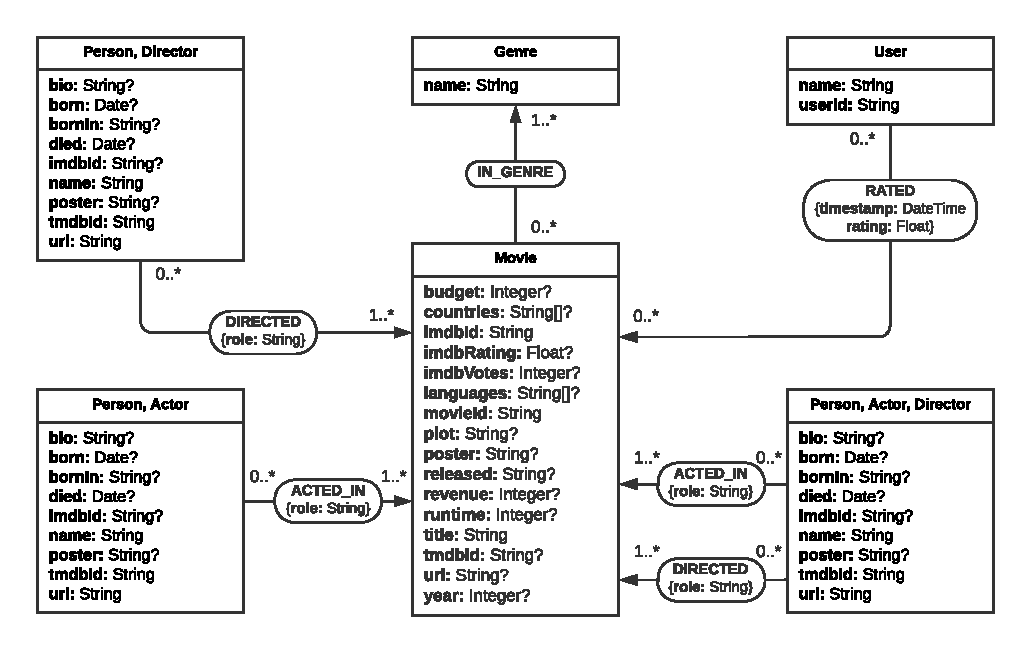
\includegraphics[width=\textwidth]{figures/schema-recommendations.pdf}
  \caption[The schema of the Recommendations Graph dataset]{The schema of the Recommendations Graph dataset. This schema was constructed manually by analyzing the data.}
  \label{fig:schema-recommendations}
\end{figure}

\begin{figure}[t]
  \centering
  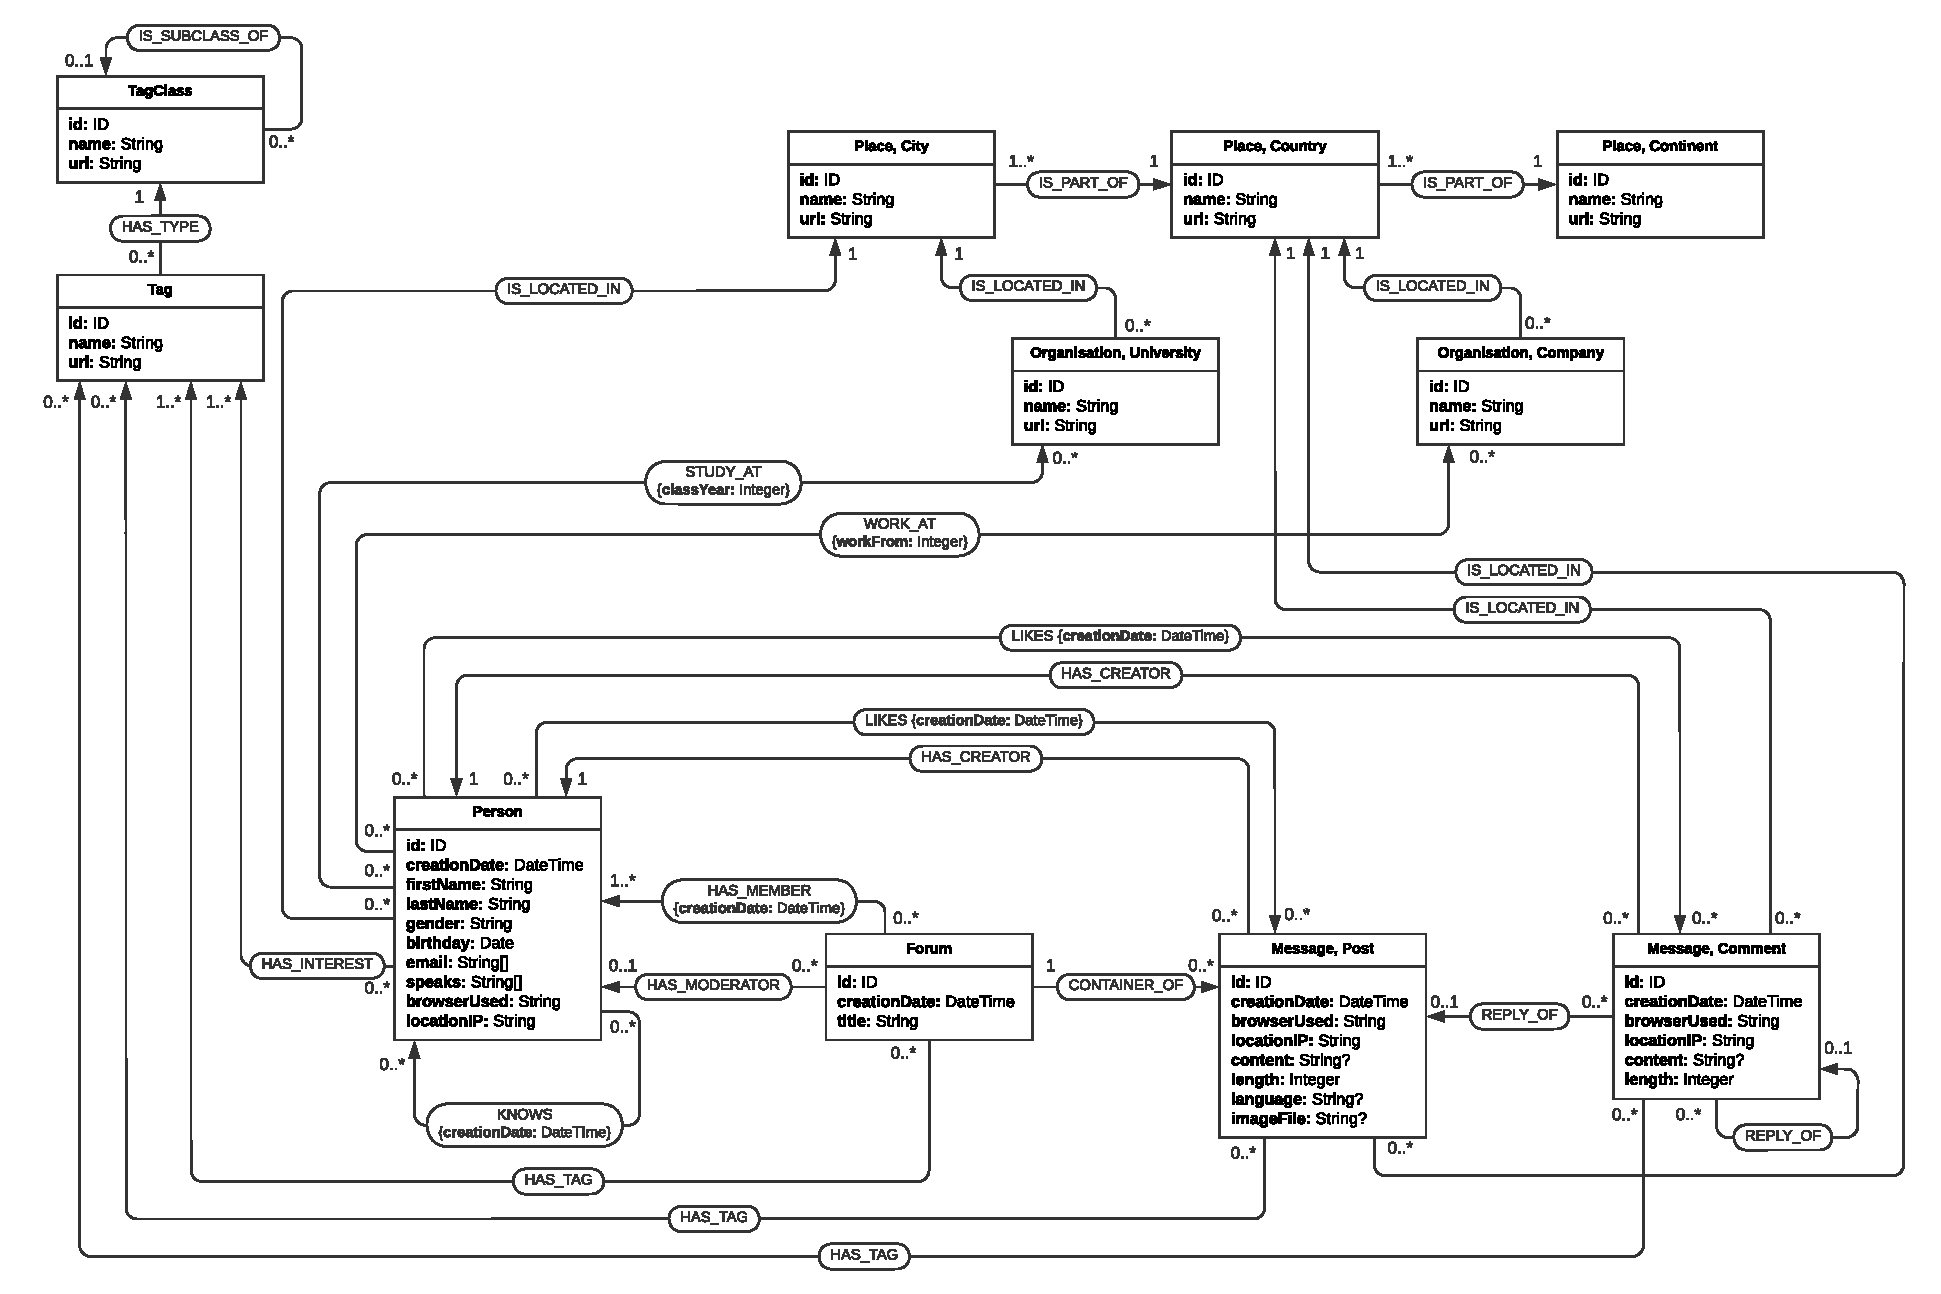
\includegraphics[width=\textwidth]{figures/schema-snb.pdf}
  \caption[The schema of the SNB dataset]{The schema of the SNB dataset. This schema was created by modifying the schema from \citet{angles2020snb} to not rely on subtype relations. Because our schema formalism does not support subtyping, the resulting schema is more permissive than the original. This limitation is discussed in detail in \autoref{ch:limitations}.}
  \label{fig:schema-snb}
\end{figure}

\paragraph{Validation variant.} As described in \autoref{sec:variants}, we consider two variants of the validation problem: binary and full validation. For binary validation, we measure the time until the first violation is found (or until the last query has finished, if there are no violations). For the full variant, we measure until the last query has finished.

\paragraph{Violation rate.} We expect the validation time of the binary variant to be affected by the number of violations in the data. If the data graph conforms to the schema, the entire graph is scanned. However, as soon as a single violation is found, it can terminate. The higher the violation rate, the sooner we expect to terminate.

We consider three levels of violation rate:

\begin{itemize}
  \item \emph{None:} the graph conforms to the schema.
  \item \emph{Single:} a single node violates a constraint.
  \item \emph{Many:} roughly 50\% of all nodes violate a constraint.
\end{itemize}

The way violations are introduced depends on the database system under test, due to their differences in schema capabilities and data model. For JanusGraph, we remove a mandatory property from nodes. Because TigerGraph requires every property to have a value, we set it to the default value instead. Because Neo4j supports constraints that prevent missing mandatory properties, we remove a mandatory edge instead. Edges are not modified, hence they do not violate any constraints.

The choice to only introduce violations on nodes is convenient, but we expect it to be sufficient to have a measurable effect. If we assume the validation process to be a random search through all objects, we can see it as a sequence of random trials with probability $1-p$, where $p$ is the proportion of objects that violate a constraint. Then, the time until the first violation is detected shrinks exponentially with the number of violations in the data. While all of our datasets have more edges than nodes, the ratio of nodes to edges is large enough to make a significant difference in theoretical binary validation time between the levels of violation rate.

\subsection{Parameters}

We control the following parameters so that they are the same for every workload.

\paragraph{Indexing and caching.} To enable a fair comparison between databases, we attempt to put an equal amount of effort into optimization for each of them. We use only indexes that the database system creates by default. Most of these are not useful to us, because their purpose is to find sets of objects with specific labels or properties. The exception is TigerGraph's outdegree index (see \autoref{sec:implementation}), which may speed up the validation of cardinality constraints. To improve independence between subsequent runs, caching is disabled for Neo4j and JanusGraph. TigerGraph does not provide any caching functionality that we know of.

\paragraph{Hardware.} All workloads are run on a single machine with 4 CPU cores, 6 gigabytes of dedicated memory, and a solid-state drive with enough capacity to store all data.

\section{Results}

In this section, we show the results of our experiments. We attempt to answer each research question using plots and statistical tests. The complete set of results is available on GitHub\footnote{\url{https://github.com/nimobeeren/thesis/blob/main/analysis/results.csv}}.

\subsection{\ref*{rq:variant}: Validation Variant}

We run both the binary and full validation queries on all datasets. For these workloads, no violations are introduced. While we are also interested in the effect of violations on the binary variant, this is addressed in \autoref{sec:results-violations}. We perform an independent two-sided T-test \citep{student1908probable} to test the null hypothesis that the mean validation time is the same for the full and binary variant, with all other variables fixed. The results for each database are shown in \autoref{fig:results-variant} and \autoref{tab:results-variant}. The queries for JanusGraph on the SNB dataset with scale factor larger than 0.1 did not complete within an hour, and are not shown here.

\begin{figure}[p]
  \centering
  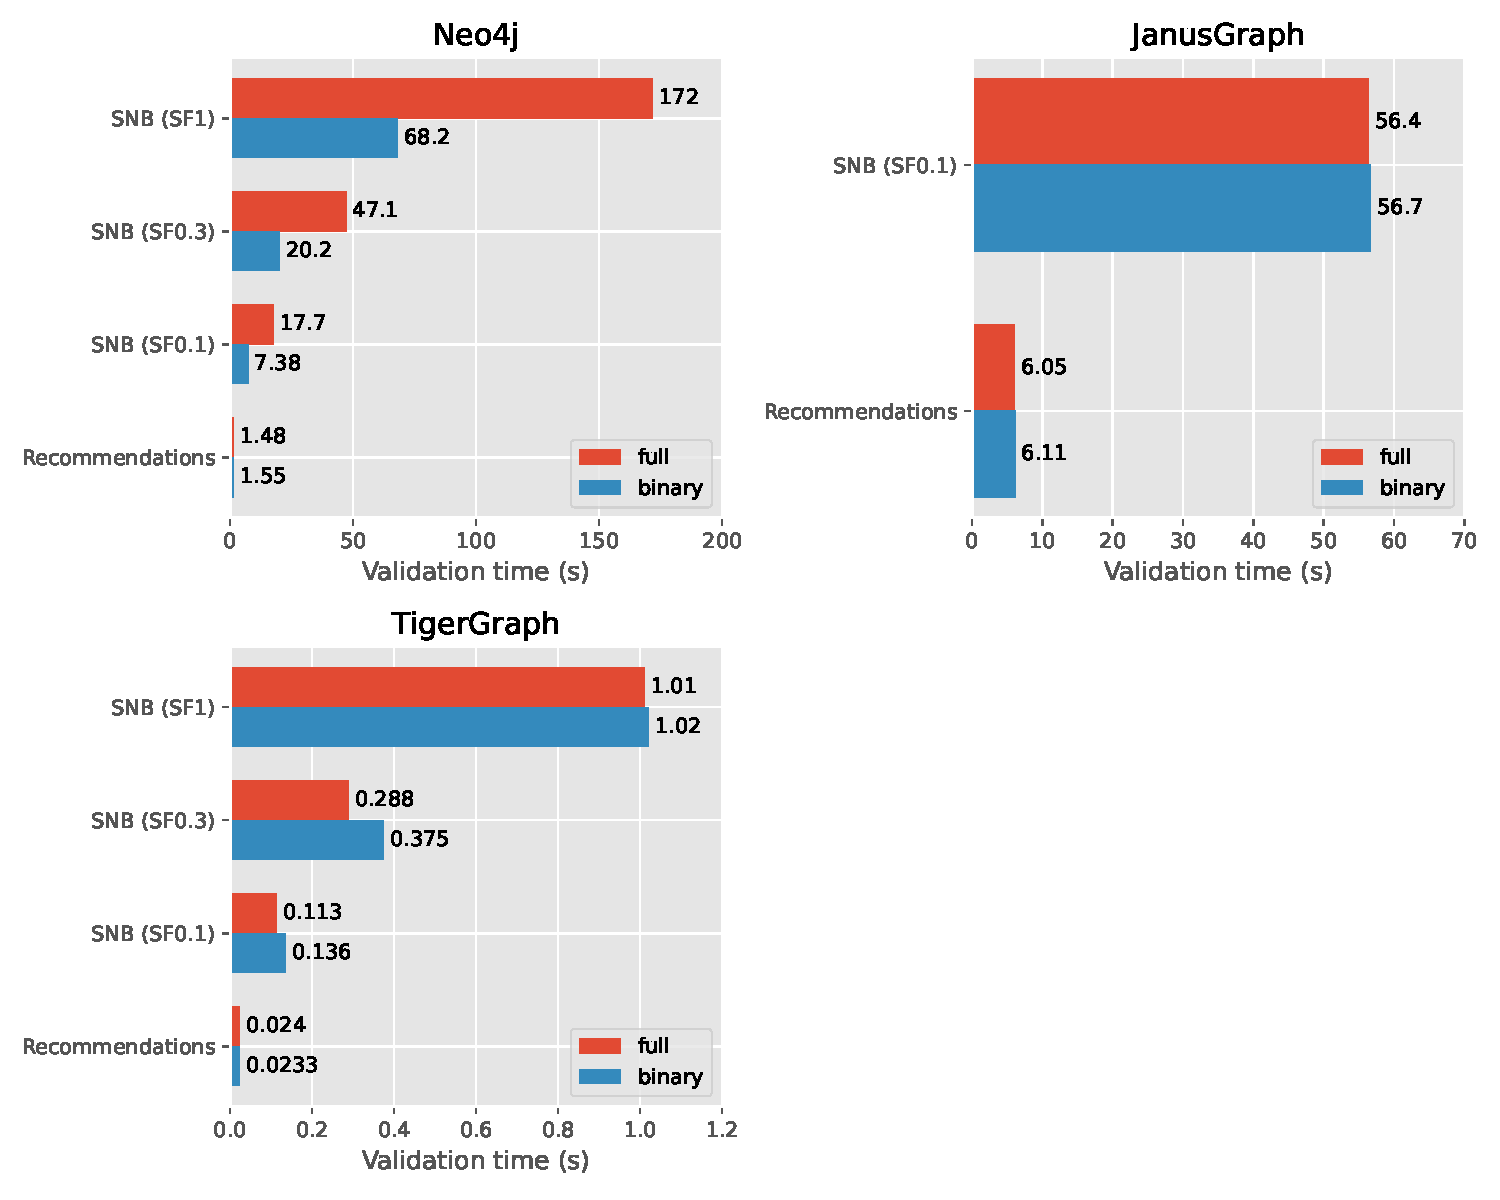
\includegraphics[scale=0.5]{figures/results-variant.pdf}
  \caption[Mean validation time for full and binary variants]{Mean validation time for binary and full variants on all datasets with no schema violations.}
  \label{fig:results-variant}
\end{figure}

\begin{table}[p]
  \centering
  \begin{tabular}{llrrrr}
    \hline
    \textbf{Database}           & \textbf{Dataset} & \multicolumn{2}{c}{\textbf{Mean validation time (s)}} & \textbf{t}      & \textbf{p}                                \\
                                &                  & \textbf{Full}                                         & \textbf{Binary} &            &                              \\
    \hline
    \multirow{4}{*}{Neo4j}      & SNB (SF1)        & 171.89                                                & 68.17           & 49.9       & $\mathbf{<}\textbf{0.0001*}$ \\
                                & SNB (SF0.3)      & 47.13                                                 & 20.18           & 28.9       & $\mathbf{<}\textbf{0.0001*}$ \\
                                & SNB (SF0.1)      & 17.71                                                 & 7.38            & 31.3       & $\mathbf{<}\textbf{0.0001*}$ \\
                                & Recommendations  & 1.48                                                  & 1.55            & -0.37      & 0.731                        \\
    \hline
    \multirow{2}{*}{JanusGraph} & SNB (SF0.1)      & 56.41                                                 & 56.74           & -0.56      & 0.608                        \\
                                & Recommendations  & 6.05                                                  & 6.11            & -0.42      & 0.697                        \\
    \hline
    \multirow{4}{*}{TigerGraph} & SNB (SF1)        & 1.01                                                  & 1.02            & -0.66      & 0.546                        \\
                                & SNB (SF0.3)      & 0.29                                                  & 0.38            & -1.34      & 0.252                        \\
                                & SNB (SF0.1)      & 0.11                                                  & 0.14            & -0.78      & 0.478                        \\
                                & Recommendations  & 0.02                                                  & 0.02            & 0.32       & 0.768                        \\
    \hline
  \end{tabular}
  \caption[Mean validation time for binary and full variants]{Mean validation time for binary and full variants on all datasets with no schema violations. A two-sided T-test is performed to test for a difference between the mean validation time for the full and binary variant. We give the \emph{t-statistic} as defined by \citet{student1908probable}, as well as the p-value. Significant results (p $< 0.05$) are marked with a *.}
  \label{tab:results-variant}
\end{table}

For Neo4j, we find a statistically significant difference (p $< 0.05$) between the full and binary variants, for all datasets except the Recommendations. This difference could be explained by the use of Neo4j's schema statistics, which are retrieved in constant time and eliminate the need for some of the queries used in the full variant. However, on the smaller Recommendations dataset this advantage is no longer apparent, possibly because the constant lookup time outweighs the time saved by skipping some queries. We do not find evidence to suggest any difference between the two variants for JanusGraph and TigerGraph. This is expected, since the queries for both variants are very similar, and the binary variant cannot terminate early because the data conforms to the schema.

\subsection{\ref*{rq:scale}: Scale}

To further illustrate the relationship between validation time and the scale of the data, \autoref{fig:results-scale} plots the validation time against the number of objects in the data graph. To keep the schema and structure constant, we only consider the SNB dataset, but at different scale factors. We do not plot the results for JanusGraph, because only the smallest scale factor could be successfully tested.

\begin{figure}[t]
  \centering
  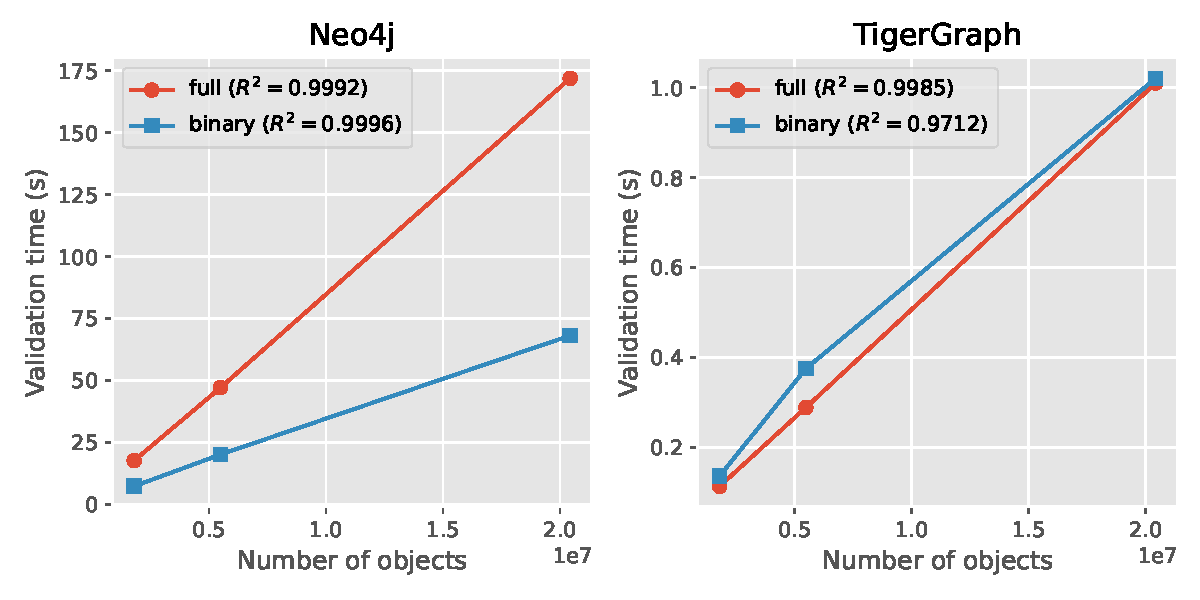
\includegraphics[scale=0.5]{figures/results-scale.pdf}
  \caption[Validation time against number of objects in the data graph]{Validation time against number of objects in the data graph for the SNB dataset with no schema violations. The markers represent individual measurements and the lines represent fitted linear regression models.}
  \label{fig:results-scale}
\end{figure}

These results suggest a linear relationship between number of objects and validation time. This conclusion is supported by fitting a simple linear regression model using the least squares method. We use the number of objects as the explanatory variable and the validation time as the response variable. The high $R^2$ values suggest a good fit. This linear relationship is expected, since our queries perform a linear scan of the nodes and edges in the data graph.

\subsection{\ref*{rq:violations}: Violation Rate}
\label{sec:results-violations}

The workloads so far have did not contain any schema violations, meaning that the data conformed to the schema. To evaluate how schema violations affect the validation time question, we choose a fixed dataset and introduce some errors into the data. We choose the SNB dataset at SF0.1, because all databases could succesfully complete full validation, and the scale is large enough to have potential for improvement. We only test the binary validation variant, because we do not expect the amount of violations to have a significant impact on the full variant. A one-way ANOVA is performed to test the null hypothesis that the mean validation time is the same for all violation rates for a particular database. The results are shown in \autoref{fig:results-violations} and \autoref{tab:results-violations}.

\begin{figure}[t]
  \centering
  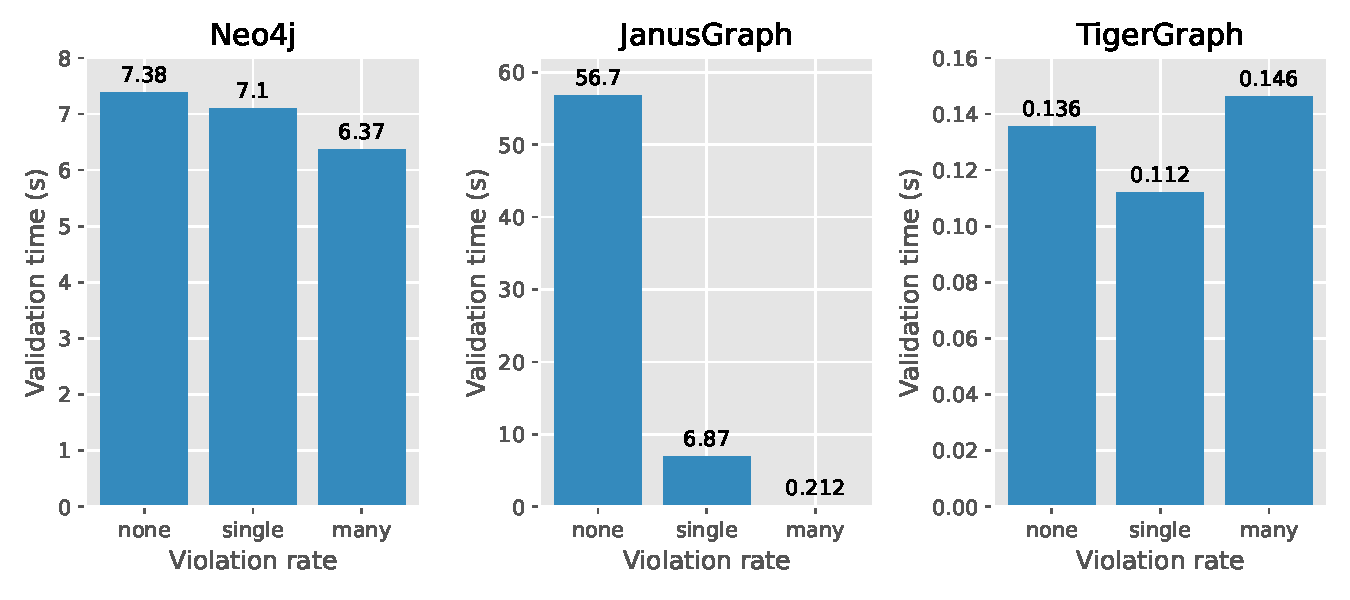
\includegraphics[scale=0.5]{figures/results-violations.pdf}
  \caption[Mean validation time at different violation rates]{Mean validation time at different violation rates for binary validation of the SNB (SF0.1) dataset.}
  \label{fig:results-violations}
\end{figure}

\begin{table}[t]
  \centering
  \begin{tabular}{lrrrrrrrrr}
    \hline
    \textbf{Database} & \multicolumn{3}{c}{\textbf{Mean validation time (s)}} & \textbf{F}      & \textbf{p}                                           \\
                      & \textbf{None}                                         & \textbf{Single} & \textbf{Many} &                                      \\
    \hline
    Neo4j             & 7.38                                                  & 7.10            & 6.37          & 14.21 & \textbf{0.005*}              \\
    JanusGraph        & 56.74                                                 & 6.87            & 0.21          & 27152 & $\mathbf{<0.0001}\textbf{*}$ \\
    TigerGraph        & 0.14                                                  & 0.11            & 0.15          & 0.55  & 0.601                        \\
    \hline
  \end{tabular}
  \caption[Mean validation time at different violation rates]{Mean validation time at different violation rates for binary validation of the SNB (SF0.1) dataset. A one-way ANOVA is performed to test for a difference between the mean validation time among all violation rates. We give the F-statistic as defined by \citet{snedecor1989statistical} as well as the p-value. Significant results (p $< 0.05$) are marked with a *.}
  \label{tab:results-violations}
\end{table}

The results show different patterns for each database. For Neo4j, increasing the violation rate decreases validation time, but not by a large amount. For JanusGraph, even a single violation cuts the validation time by an order of magnitude, and when half of all nodes violate a constraint, validation time is again significantly reduced. For TigerGraph, we found no evidence that increasing the violation rate reduces validation time.

The different patterns could be explained by the order in which different kinds of violations are checked in our queries. Recall that in Neo4j, we introduce violations by removing mandatory edges. This happens to be the last thing that is checked in our validation queries, hence all other checks still need to be completed. The fact that there is any improvement at all does suggest that Neo4j recognizes it can terminate the query as soon as it finds a violation. For JanusGraph, we only need two queries: the first checks all nodes and the second checks all edges. Since the violation always appears in one of the nodes, the edge query can be skipped. This yields significant time gains, since there are roughly 5 times more edges than nodes. By contrast, TigerGraph shows no indication of improvement when introducing violations, which suggests that it does not terminate early.

\subsection{\ref*{rq:database}: Database}

From the previous results, we can see there is a clear difference in performance between database systems. In nearly all scenarios, TigerGraph beats Neo4j by an order of magnitude, and JanusGraph is another order of magnitude slower. The only exception occurs when we introduce violations to the data. When there is a single violation, JanusGraph's performance is roughly equal to Neo4j's, and when there are many violations, JanusGraph is on par with TigerGraph.

We are hesitant to draw conclusions about the optimal level of performance that could be achieved with better optimizations specific to each database, since indexes and other optimizations can have a large impact on execution time. However, these results give an indication of the level of performance that can be expected from an initial implementation.

\chapter{Limitations and Future Work}
\label{ch:limitations}

\section{Schema Formalism}

We discuss limitations and opportunities for improvement of our schema formalism as defined in \autoref{ch:pg-schema}.

\paragraph{Subtyping.} \citet{barker1990entity} introduced the concept of subtyping to the ER model, \citet{lbath2021inference} included subtyping in their schema inference method, and we have seen subtype relations appearing in the SNB property graph schema (\autoref{fig:schema-snb}). Clearly, there is a need for subtyping in property graph schemas. This would help model domains containing type hierarchies more accurately, and would reduce duplication of schema edges and properties.

In general, subtype relations cannot be expressed using our formalism. The problem is illustrated by the schema depicted in \autoref{fig:subtyping}. How could we express this using our schema formalism? An attempt is given in \autoref{fig:subtyping-ours}, where properties of the supertype \texttt{Message} are copied and distributed over all its subtypes, and the edge from \texttt{Comment} to \texttt{Message} is accompanied by an edge from \texttt{Comment} to Post and from \texttt{Comment} to itself. While the properties are modeled correctly in this case, it breaks down when we look at the cardinalities.

In \autoref{fig:subtyping}, a constraint is specified which we can express in words as ``every \texttt{Comment} is a reply of exactly one \texttt{Message} (or a subtype of \texttt{Message})''. However, it is not possible to specify such a constraint without subtype relations, as illustrated by \autoref{fig:subtyping-ours}. This solution allows \texttt{Comment}s which are not a reply to anything, or which are a reply to more than one thing. Then again, if we disregard the cardinality constraints, the two schemas are equivalent. This example shows that our schema formalism can be used to model some but not all subtype relations.

\begin{figure}[t]
  \centering
  \begin{subfigure}[t]{0.45\textwidth}
    \centering
    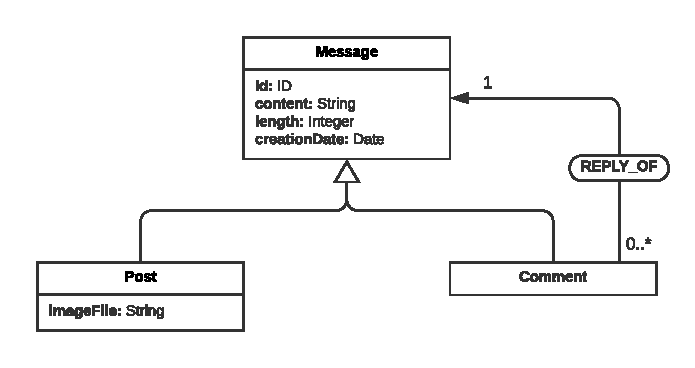
\includegraphics[width=\textwidth]{figures/subtyping.pdf}
    \caption{A schema with a subtype relation. The arrow with a solid white head indicates a ``subtype of'' relation.}
    \label{fig:subtyping}
  \end{subfigure}
  \hfill
  \begin{subfigure}[t]{0.45\textwidth}
    \centering
    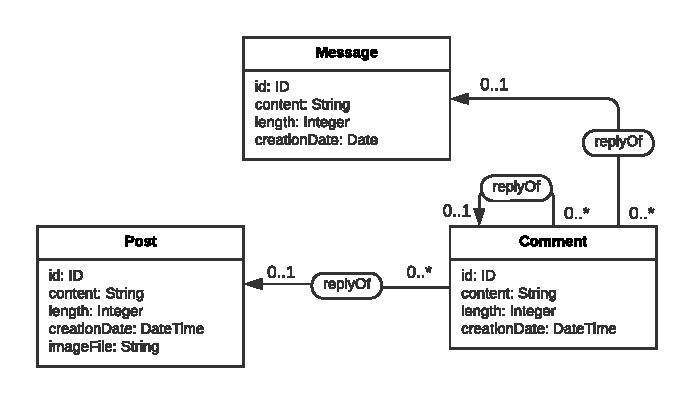
\includegraphics[width=\textwidth]{figures/subtyping-ours.pdf}
    \caption{An attempt to express the same schema without subtype relations. Note that this schema is strictly more permissive than~(a).}
    \label{fig:subtyping-ours}
  \end{subfigure}
  \caption[A schema containing subtype relations which cannot be modeled using our schema formalism]{A schema consisting of a supertype with two subtypes which cannot be modeled using our schema formalism. Any property graph that conforms to~(a) also conforms to~(b), but not the other way around.}
\end{figure}

\paragraph{Larger graph patterns.} It is not possible to specify constraints over a graph pattern larger than two neighboring nodes and the edge between them. For example, say we want to allow a person to drive a car, but only when they have a driver's license. \autoref{fig:drivers-license} depicts a schema that models these entities and their relations using three nodes and two edges. Unfortunately, it is not possible to prevent a person from driving a car without having a driver's license. This illustrates the limited scope of the constraints that we can specify.

\begin{figure}[t]
  \centering
  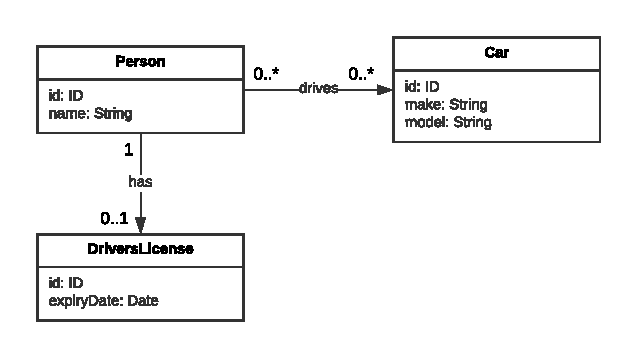
\includegraphics{figures/drivers-license.pdf}
  \caption[A schema illustrating a larger graph pattern constraint which cannot be captured by our schema formalism]{A schema illustrating a larger graph pattern constraint which cannot be captured by our schema formalism. While we can specify constraints on edge cardinalities, we cannot ensure that a person only drives a car if they have a driver's license.}
  \label{fig:drivers-license}
\end{figure}

\paragraph{Key constraints.} Our schema formalism does not support property uniqueness or key constraints. While key constraints were already present in ER models \citep{chen1976entity}, their application to property graphs is non-trivial. As argued in the \textsc{PG-Keys} proposal \citep{angles2021keys}, there is a need for granular and flexible key constraints. Keys should be applicable to nodes, edges, and properties, which could all represent concrete entities. Moreover, key scopes and descriptors should be defined in a way that allows objects to be keyed by their relations to other objects. Finally, keys may be \emph{exclusive}, \emph{mandatory}, \emph{singleton}, or any combination thereof. Future work should consolidate \textsc{PG-Keys} with a comprehensive schema formalism such as ours.

\paragraph{Mutual exclusivity.} Another kind of constraint introduced by \citet{barker1990entity} is mutual exclusivity of edges. For example, a \texttt{Person} may have a \texttt{WORKS\_AT} edge to a \texttt{Bank} or a \texttt{TradingCompany}, but not both. Mutual exclusivity could be incorporated into our schema formalism, though we should carefully consider whether the benefits for users weigh up against the added complexity. Some constraints may be easier to understand and implement efficiently through seperate queries or another constraint language that sits on top of our schema validation queries.

\section{Empirical Evaluation}

We discuss limitations and threats to the validity of our experiments of \autoref{ch:experiment}.

\paragraph{Internal validity.} This concerns the degree of confidence in the causal relationships which we inferred from our results. The way we measured validation time poses a threat to internal validity, because the instrumentation differed between databases. For Neo4j and TigerGraph, we rely on the query logs to yield an accurate measurement, while for JanusGraph we use the wall-clock time. The method of time measuring might create some variance between databases, although this can only explain a small part of the difference we observed.

Furthermore, some variance in validation time can be explained by background processes and low-level CPU optimizations. We suspect this factor to have a small impact, though possibly significant when measuring on a sub-second timescale.

\paragraph{Construct validity.} This concerns the way our variables of interest were operationalized. One threat to construct validity comes from the way we introduced schema violations into the data. This was done by either removing a mandatory property or a mandatory edge for a node (depending on the database). In reality, different kinds of violations could occur: extraneous properties, incorrect datatypes, or incorrect edge cardinality and others. These could have differing effects on validation time.

\paragraph{External validity.} This concerns the generalization of our results. One such threat comes from the scale of the datasets used in our experiment, which ranged from roughly 200K to 20M objects. We observed a linear relationship between the number of objects and the validation time. However, this relationship may not generalize to very large datasets, especially when they are too large to fit on a single disk.

Another threat to external validity arises from the two schemas we have analyzed (Recommendations and SNB). The number of schemas is limited, and we did not perform any experiments to isolate the effect of different schemas. Moreover, the schemas are similar in terms of the kinds of constraints they express. Neither of the schemas contain cardinality constraints of the form ``exactly~$n$'', even though this can be expressed with our schema formalism. Future work could investigate the relationship between validation time and schema size or the kinds of constraints in the schema. This could be done by validating the same datasets against several schemas.

Finally, it is unclear whether the differences between databases would persist when further optimizations are made. We tried to put equal effort into optimization for each database, but results may differ when more labor is exerted.

\section{Miscellaneous}

\paragraph{Generic validation implementation.} In our approach, the validation queries are hand-crafted for each schema. This requires knowledge of the query language and the schema functionality of a particular database. To make things easier for the user, we could let them provide a schema in a generic schema language or diagram, and generate the validation queries instead.

Alternatively, when the schema and data are both given as graphs, validation could be achieved using generic graph pattern matching queries. In fact, we have provided such a generic implementation for Neo4j\footnote{\url{https://github.com/nimobeeren/thesis/tree/main/neo4j/generic}}. Unfortunately, validation times were prohibitive for all but the smallest graphs. However, there are certainly opportunities for performance gains.

\paragraph{Validation algorithms.} There are advantages to our approach using graph queries for validation: they are easy to adjust, portable between database versions, and convenient to prototype. However, when performance is the primary goal, a lower-level implementation may be more suitable. Specialized validation algorithms and indexes could be developed to achieve performance benefits. Moreover, since all of our validation rules have a limited scope, validation queries may be parallelized and distributed across multiple machines.

If a database instance is frequently updated, the cost of scanning the entire graph on every update may be prohibitive. In such a scenario, an incremental validation algorithm could provide significant benefits. Due to the limited scope of our validation rules, only the fragment of the graph that is affected by the update would need to be revalidated. Such an algorithm could be used to reject any updates that cause a schema violation.

\paragraph{Schema-aware query optimization.} Schema knowledge may be used by the query engine to improve query planning. Such optimizations are widely employed in relational databases \citep{chakravarthy1990logic, meier2013semantic,silberschatz2011database}, and have been studied in the context of graph databases as well \citep{buneman1997adding,popa1999equational}. Similar methods could be applied to property graph databases when a schema is present.

\paragraph{Query type checking and inference.} The presence of schemas may benefit the usability of graph databases. Through query type checking, incorrectly typed parameters could be detected. Moreover, the result type of a query could be inferred to ensure the result is of the expected type before execution. Query type inference could be integrated with type systems of programming languages to achieve type safety across the database and the application. A type inference approach like the one presented by \citet{colazzo2015typing} may be adapted to the property graph model.

\paragraph{Relation to other notions of schema conformance.} It may be of theoretical interest to investigate how our notion of conformance is related to other methods found in the literature, such as simulation \citep{buneman1997adding} and homomorphisms \citep{bonifati2019schema}. If they are equivalent, results from other work may be applied to our model as well.

\chapter{Conclusion}

% TODO: conclusion

\bibliography{main}

\end{document}
